\documentclass[a4paper,11pt,notitlepage]{report}

\usepackage{graphicx}
\usepackage[utf8]{inputenc}
\usepackage[T1]{fontenc}
\usepackage[ngerman]{babel}
\usepackage{bibgerm}
\usepackage{amsmath,amssymb,amsthm}
\usepackage{color}
\usepackage{enumerate}
\usepackage{tabularx}
\usepackage{subfig}
\usepackage{fancyhdr}
\usepackage{upgreek}
\usepackage[pdftex,pdfpagelabels,colorlinks,backref,pagebackref]{hyperref}
\usepackage{tikz} % SELBST HINZUGEFÜGT
\usepackage{lmodern}
\usepackage{subfig}
\usepackage{stmaryrd}
\usepackage{shadethm}
% == Set the heading style ===================================================
\setlength{\headheight}{14pt}
\pagestyle{fancyplain}
\renewcommand{\chaptermark}[1]{\markboth{#1}{}}
\renewcommand{\sectionmark}[1]{\markright{\thesection\ #1}}
\lhead[\fancyplain{}{\thepage}]{\fancyplain{}{\rightmark}}
\rhead[\fancyplain{}{\leftmark}]{\fancyplain{}{\thepage}}
\cfoot{}
\renewcommand{\headrulewidth}{0.4pt}
% ============================================================================

% == Set correct values for fitting floats ===================================
\tolerance=2000
\emergencystretch=10pt

\setcounter{topnumber}{3}
\setcounter{totalnumber}{5}
\setcounter{bottomnumber}{2}

% To make those darn floats fit where they should
\setcounter{totalnumber}{9}
\setcounter{topnumber}{9}
\setcounter{bottomnumber}{9}
\renewcommand{\textfraction}{0.00}
\renewcommand{\topfraction}{1.0}
\renewcommand{\bottomfraction}{1.0}
% ============================================================================

% == German definitions for theorems etc. ==================================== 
\theoremstyle{definition}
\newshadetheorem{definition}{Definition}[chapter]
\newshadetheorem{theorem}{Satz}[chapter]
\newtheorem{lemma}{Lemma}[chapter]
\newtheorem{proposition}{Proposition}[chapter]
\newtheorem{corollary}{Korollar}[chapter]
\newtheorem{observation}{Beobachtung}[chapter]
\newtheorem{fact}{Fakt}[chapter]
\newtheorem{remark}{Bemerkung}[chapter]
\newtheorem{example}{Beispiel}[chapter]
\newtheorem{beh}{Behauptung}[chapter]
% ============================================================================

% == Abkürzungen für die reellen, natürlichen, ganzen,... Zahlen =============
\newcommand{\R}{{\ensuremath{\mathbb{R}}}}
\newcommand{\N}{{\ensuremath{\mathbb{N}}}}
\newcommand{\Z}{{\ensuremath{\mathbb{Z}}}}
\newcommand{\C}{{\ensuremath{\mathbb{C}}}}
\newcommand{\Q}{{\ensuremath{\mathbb{Q}}}}
\newcommand{\F}{{\ensuremath{\mathbb{F}}}}
\newcommand{\Prim}{{\ensuremath{\mathbb{P}}}}
% ============================================================================

% == Makros für Autorenname und -adresse =====================================
\newcommand{\myaddress}[6]{%
  \parbox{\textwidth}{\textbf{\large #1}\\
    #2\\ #3\\ #4\\ 
    \ifthenelse{\equal{#5}{}}{}{Email: \href{mailto:#5}{\texttt{#5}}\\}
    \ifthenelse{\equal{#6}{}}{}{WWW: \href{#6}{\path|#6|}\\}
  } 
}

\newcommand{\myauthor}[1]{%
  \addtocontents{toc}{\protect\hspace{3.35ex}%
  \textsl{#1}\par}\vspace{-4ex}\quad\hfill\textsl{\Large #1}\vspace{8ex}}

\newcommand{\myname}[1]{\Large #1}

\title{\textbf{{Einführung in die Geometrie und Topologie - Mitschrieb -} \\[5ex] 
    {\Large Übung im Wintersemester 2011/2012\\[5ex]}}}

%%%%%%%%%%%%%%%%%%%%%%%%%%%%%%%%%%%%%%%%%%%%%%%%%%
% Tragen Sie in der folg. Zeile Ihren Namen ein: %
%%%%%%%%%%%%%%%%%%%%%%%%%%%%%%%%%%%%%%%%%%%%%%%%%%
\author{\myname{Sarah Lutteropp, Simon Bischof}}

\newcommand{\RM}[1]{\MakeUppercase{\romannumeral #1{}}} 
\newcommand{\OO}{{\ensuremath{\mathcal{O}}}}

\begin{document}
\shorthandoff{"}
\begin{titlepage}
	\begin{center}	
		\LARGE \textbf{{Einführung in die Geometrie und Topologie - Mitschrieb -} \\[5ex] 
    		{\Large Übung im Wintersemester 2011/2012\\[5ex]}}
	\end{center}
	\begin{center}
		\Large Sarah Lutteropp, Simon Bischof
	\end{center}
	\begin{center}
		\today
	\end{center}
	\vspace{2cm}
	\begin{center}
		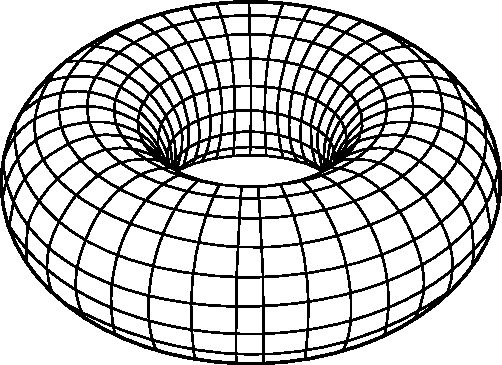
\includegraphics[width=0.8\textwidth]{torus2.pdf}
	\end{center}
\end{titlepage}
%\maketitle
\setcounter{tocdepth}{1}
\tableofcontents

\section*{Vorwort}
Dies ist ein Mitschrieb der Übung “Einführung in die Geometrie und Topologie” vom Wintersemester 2011/2012 am Karlsruher Institut für Technologie, die von Frau Dipl.-Math. Sandra Lenz gehalten wird.

\chapter{24.10.2011}

\begin{section}{Induzierte Topologie}
	\begin{definition}[Induzierte Topologie]
		Sei $X$ eine Menge. Sei $d \colon X \times X \rightarrow \R$ eine Metrik. Diese Metrik $d$ definiert durch folgende Bedingung eine Topologie $\OO$ auf $X$:
		\newline
		$O \subseteq X$ ist genau dann offen (d.h. $O \in \OO_d$), wenn für alle $x \in O$ ein $\epsilon > 0$ existiert mit
		$$
			B_\epsilon (x) := \{y \in X \mid d(x,y) < \epsilon\} \subseteq O.
		$$
		($B_\epsilon$ nennt man offenen $\epsilon$-Ball.)
	\end{definition}
\end{section}

\begin{section}{Offen und abgeschlossen}
	Sei $X$ eine Menge.
	\begin{itemize}
		\item Mengen können sowohl offen als auch abgeschlossen (zugleich) sein.
			\begin{example}
				Betrachte $\emptyset$ und $X$ in der trivialen Topologie $\OO = \{X, \emptyset\}$.
					\newline
					Es gilt: $X \in \OO, \emptyset \in \OO$ nach Definition, d.h. $X$ und $\emptyset$ sind offen.
					\newline
					Außerdem gilt: $X^c = \emptyset \in \OO$, ebenso: $\emptyset^c = X \in \OO$, d.h. die Komplemente von $X$ und $\emptyset$ sind offen und somit $X$ und $\emptyset$ abgeschlossen.
			\end{example}
			
		\item Mengen können weder offen noch abgeschlossen sein.
			\begin{example}
				Betrachte $\R$ mit der von der Standardmetrik induzierten Topologie. Es ist $[0,1[$ nicht offen in dieser Topologie, denn für den Punkt $0$ finden wir kein $\epsilon > 0$, so dass $B_\epsilon(0)$ in $[0,1[$ liegt.
				Die Menge $[0,1[$ ist aber auch nicht abgeschlossen, da ihr Komplement $\R \backslash [0,1[ = ]-\infty,0[ \cup [\underline{1},\infty[$ nicht offen ist.
			\end{example}
		\item Bilder offener Mengen unter stetigen Abbildungen müssen nicht notwendigerweise offen sein.
			\begin{example}
				Betrachte $\R$ mit der von der Standardmetrik induzierten Topologie.
				\newline
				Definiere $f \colon \R \rightarrow \R, x \mapsto x^2$.
				\newline
				Es gilt für die in $\R$ offene Menge $]-1,1[$:
				\newline
				$f(]-1,1[)=[0,1[$ und $[0,1[$ ist nicht offen in $\R$.
			\end{example}
	\end{itemize}
\end{section}

\begin{section}{Basis der von der Standardmetrik auf dem $\R^n$ definierten Topologie}
	$$\mathcal{B} = \{B_{\frac{1}{m}}(x) \mid x \in \Q^n, m \in \N\}$$
	Diese Basis ist abzählbar.
\end{section}

\begin{section}{Teilraumtopologie}
	Es sei $(X, \OO)$ ein topologischer Raum, $A \subseteq X$.
	\newline
	Die Teilraumtopologie (oder Spurtopologie) ist definiert durch
	$$\OO \big |_{A} := \{U \cap A \mid U \in \OO\} $$
	
	\begin{theorem}
		In der Tat definiert $\OO \big |_{A}$ eine Topologie auf $A$.
	\end{theorem}
	
	\begin{proof}
			$\bullet$\underline{z.z.}: Für jede Indexmenge $I$ gilt:
				$\forall i \in I \colon O_i \in \OO \big |_{A} \Rightarrow \bigcup\limits_{i \in I}{O_i} \in \OO \big |_{A}.$
			\newline
			Sei $I$ beliebige Indexmenge. Für alle $i \in I$ mit $O_i \in \OO \big |_{A}$ gilt:
			Es existieren $\mathcal{U}_i \in \OO$ mit $O_i= \mathcal{U}_i \cap A$.
			Es gilt:
			$$\bigcup\limits_{i \in I}{O_i} = \bigcup\limits_{i \in I}{(\mathcal{U}_i \cap A) } = (\bigcup\limits_{i \in I}{\mathcal{U}_i})\cap A \in \OO \big |_{A}$$ (da $\bigcup\limits_{i \in I}{\mathcal{U}_i} \in \OO$).
			\newline
			$\bullet$ \underline{z.z.}: $\forall O_1, O_2 \in \OO \big |_{A} \colon O_1 \cap O_2 \in \OO \big |_{A}.$
			\newline
			Seien $O_1, O_2 \in \OO \big |_{A}$. Dann ex. $\mathcal{U}_1, \mathcal{U}_2 \in \OO$ mit $O_i = \mathcal{U}_i \cap A, i \in \{1,2\}.$ Es gilt:
			$O_1 \cap O_2 = (\mathcal{U}_1 \cap A) \cap (\mathcal{U}_2 \cap A) = (\mathcal{U}_1 \cap \mathcal{U}_2) \cap A \in \OO \big |_{A} \text{, da } \mathcal{U}_1 \cap \mathcal{U}_2 \in \OO.$
			\newline
			$\bullet$ \underline{z.z.}: $A, \emptyset \in \OO \big |_{A}.$
			\newline
			Es gilt: $A = X \cap A \in \OO \big |_{A}\text{, da } X \in \OO$ nach Definition von $\OO$. 
			\newline
			Es gilt: $\emptyset = \emptyset \cap A \in \OO \big |_{A} \text{, da } \emptyset \in \OO$ nach Definition von $\OO$.
	\end{proof}
\end{section}

\begin{section}{Homotopieäquivalenz}
	\begin{definition}
		Seien $X,Y$ topologische Räume. $X$ heißt \underline{homotopieäquivalent zu Y}, falls es stetige Abbildungen $f \colon X \rightarrow Y$ und $g \colon Y \rightarrow X$ gibt, so dass $f \circ g \simeq id_Y$ und $g \circ f \simeq id_X$.
	\end{definition}
	
	\begin{theorem}
		$\R^n \backslash \{0\}$ ist homotopieäquivalent zur Sphäre $S^{n-1}$.
	\end{theorem}
	
	\begin{proof}
		Sei $f \colon S^{n-1} \hookrightarrow \R^n \backslash \{0\}, x \mapsto x$ (Inklusionsabbildung). Dann ist $f$ stetig.
		\newline
		Sei weiter $g \colon \R^n \backslash \{0\} \rightarrow S^{n-1}, x \mapsto \frac{x}{||x||}$. Dann ist auch $g$ stetig und es gilt:
		$g \circ f = id_{S^{n-1}}$, also insbesondere $g \circ f \simeq id_{S^{n-1}}$.
		\newline
		Für $f \circ g$ betrachte folgende Abbildung:
		$$H \colon \R^n \backslash \{0\} \times [0,1] \rightarrow \R^n \backslash \{0\}, (x,t) \mapsto (1-t) \frac{x}{||x||} + t \cdot x$$
		Dann ist $H$ stetig und es gilt für alle $x \in \R \backslash \{0\}$:
		\newline
		$H(x,1) = x = id_{\R^n \backslash \{0\}}(x)$
		\newline
		$H(x,0) = \frac{x}{||x||} = (f \circ g)(x)$
		\newline
		Dann ist $H$ Homotopie von $f \circ g$ nach $id_{\R^n \backslash \{0\}}$ (in Zeichen: $f \circ g \simeq id_{\R^n \backslash \{0\}}$).
	\end{proof}
\end{section}

\chapter{31.10.2011}
\section{Universelle Eigenschaft der Teilraumtopologie}
Es sei $(X, \OO_X)$ ein topologischer Raum und $A \subseteq X$ versehen mit der Teilraumtopologie $\OO_A = \{ O \cap A \mid O \in \OO_X \}$. 
Weiter sei $\iota \colon A \hookrightarrow X$ die Inklusionsabbildung und $(Y, \OO_Y)$ ein weiterer topologischer Raum.

\begin{theorem}{Behauptung}
Eine Abbildung $\phi \colon Y \rightarrow A$ ist genau dann stetig, wenn die Komposition $\iota \circ \phi \colon Y \rightarrow X$ stetig ist.
\end{theorem}
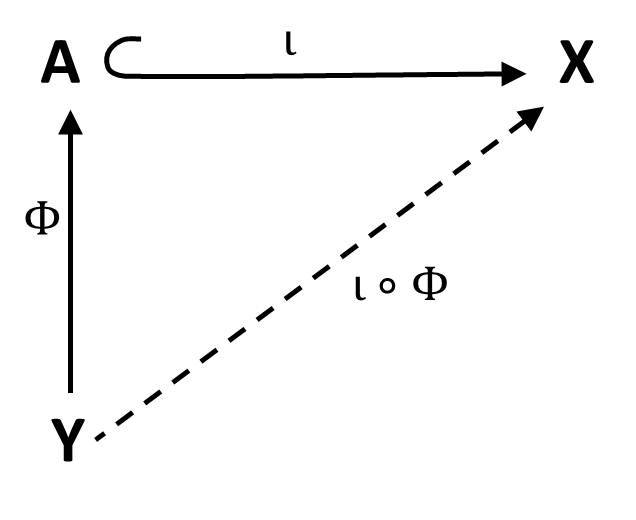
\includegraphics[width=0.4\textwidth]{images/Universell_Diagramm.jpg}
\begin{proof}
`$\Rightarrow$': Es sei $\phi \colon Y \rightarrow A$ stetig. [\underline{z.z.}: $\iota \circ \phi$ ist stetig, d.h. $\forall O \in \OO_X \colon (\iota \circ \phi)^{-1}(O) \in \OO_Y$]
\newline
Sei $O \in \OO_X$. Dann gilt $(\iota \circ \phi)^{-1}(O) = \phi^{-1}\left(\iota^{-1}(O)\right)$ und es ist $\iota^{-1}(O) \in \OO_A$, da $\iota$ stetig ist.
\newline
Es gilt somit $\phi^{-1}\left(\iota^{-1}(O)\right) \in \OO_Y$, da $\phi$ stetig ist (nach Voraussetzung).
\newline
`$\Leftarrow$': Es sei $\phi \colon Y \rightarrow A$ eine Abbildung, so dass $\iota \circ \phi \colon Y \rightarrow X$ stetig ist. [\underline{z.z.}: $\phi$ ist stetig, d.h. $\forall O \in \OO_A \colon \phi^{-1}(O) \in \OO_Y$.]
\newline
Sei also $O \in \OO_A$. Dann existiert $O^\prime \in \OO_X$, so dass $O = O^\prime \cap A$.
Es gilt: $\iota^{-1}(O^\prime) = O^\prime \cap A = O$.
\newline
$\phi^{-1}(O) = \phi^{-1}(O^\prime \cap A) = \phi^{-1}\left(\iota^{-1}(O^\prime)\right) = (\iota \circ \phi)^{-1}(O^\prime) \in \OO_Y$, da $\iota \circ \phi$ stetig (nach Voraussetzung).
\end{proof}

\begin{remark}{(Bemerkung in der Vorlesung)}

Die Teilraumtopologie ist die gröbste Topologie, bezüglich der die Inklusionsabbildung $\iota \colon A \hookrightarrow X$ stetig ist.
\end{remark}

\begin{proof}
\underline{Stetigkeit der Inklusionsabbildung}: [\underline{z.z.}: $\forall O \in \OO_X \colon \iota^{-1}(O) \in \OO_A$]
\newline
Sei $O \in \OO_X$. Dann gilt $\iota^{-1}(O)=O \cap A \in \OO_A$.
\end{proof}


\begin{proof}
\underline{Nichtstetigkeit in gröberen Topologien}: [\underline{z.z.}: $\OO_A \not\subseteq \tilde \OO \Rightarrow \exists O^\prime \in \OO_X \colon \iota^{-1}(O^\prime) \notin \tilde \OO$]
\newline
Sei $\OO_A \not\subseteq \tilde \OO \Rightarrow \exists O \in \OO_A\colon O \notin \tilde\OO$. Dann  $\exists O^\prime \in \OO_X \colon O = O^\prime \cap A$. Damit ist aber $\iota^{-1}(O^\prime)=O^\prime \cap A = O \notin \tilde\OO \Rightarrow \iota\colon (A,\tilde\OO) \rightarrow (X,\OO_X)$ ist nicht stetig.
\end{proof}

\section{Homöomorphismen}
Zeigen Sie, dass für $a,b \in \R$ mit $a < b$ das Intervall $(a,b)$ homöomorph zum Intervall $(0,1)$ ist, sowie dass $(0,1)$ homöomorph ist zu $\R$.
\newline
Definiere $f \colon (a,b) \rightarrow (0,1), x \mapsto \frac{a-x}{a-b}$, und $g \colon (0,1) \rightarrow (a,b), x \mapsto (1-x) \cdot a + x \cdot b$.
\newline
Es gilt für alle $x \in (a,b)$:
\newline
$(g \circ f)(x) = g \left(\frac{a-x}{a-b}\right) = \left(1- \frac{a-x}{a-b}\right)a + \frac{a-x}{a-b}b = \left(\frac{a-b-a+x}{a-b}\right)a+ \frac{a-x}{a-b}b = \frac{x-b}{a-b}a + \frac{a-x}{a-b}b = \frac{ax-ab+ab-bx}{a-b} = x$.
\newline
Es gilt für alle $x \in (0,1)$:
\newline
$(f \circ g)(x)=f\left((1-x) \cdot a + x \cdot b\right)=\frac{a-((1-x)a+bx)}{a-b}=\frac{a-a+ax-bx}{a-b}=x$. Somit ist $f$ bijektiv. 
Da $f$ und $g = f^{-1}$ stetig sind, gilt damit: $f$ ist ein Homöomorphismus, d.h. $(a,b) \equiv (0,1)$.
\newline
Definiere $h \colon (0,1) \rightarrow \R, x \mapsto \tan{\left((x-\frac{1}{2})\pi \right)}$.
\newline
\newline
$f \colon [0,1) \rightarrow S^1, t \mapsto e^{2\pi i t} \left(=(\cos{2 \pi t}, \sin{2 \pi t})\right)$ ist kein Homöomorphismus (da die Umkehrabbildung nicht stetig ist).

\begin{figure}[h]
\centering
\subfloat[$f$ ist stetig $\dots$]{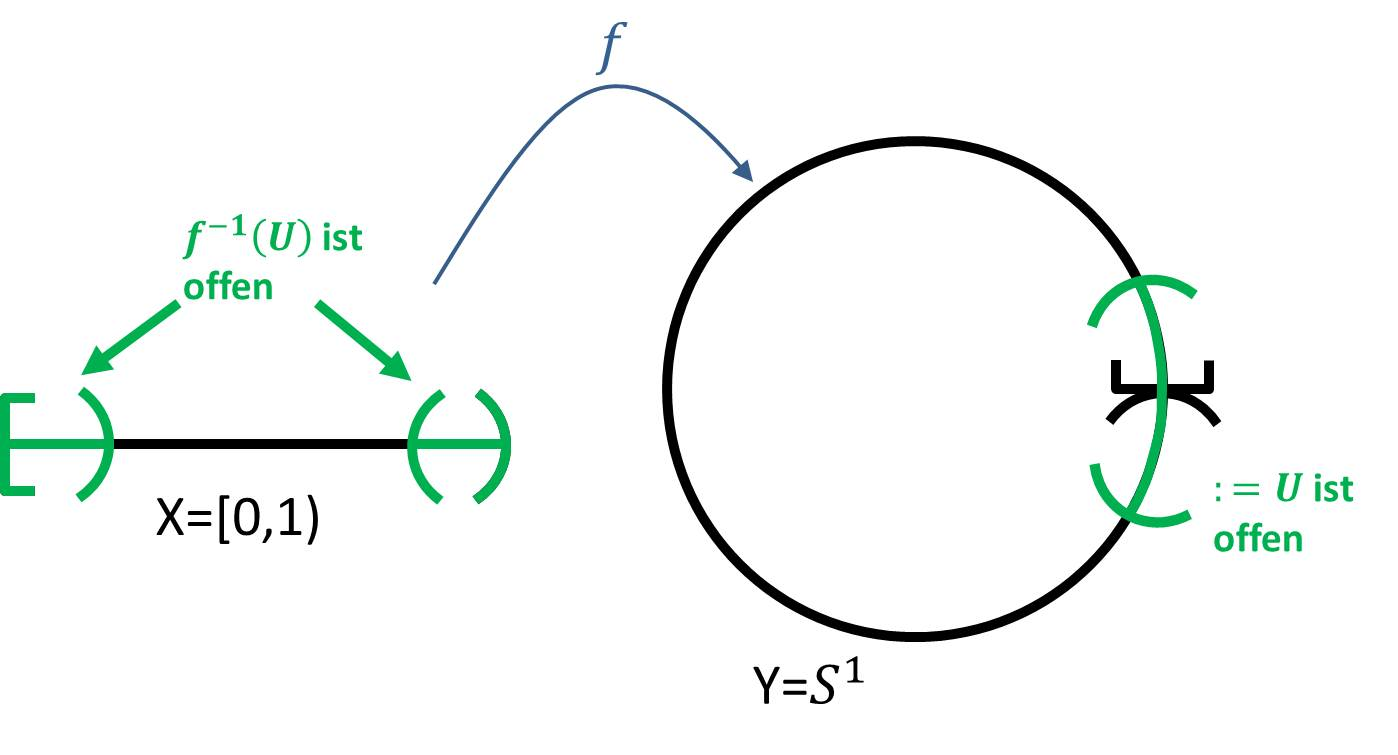
\includegraphics[width=0.75\textwidth]{images/0_1_nach_S1_f_stetig.jpg}}
\subfloat[$\dots f^{-1}$ aber nicht.]{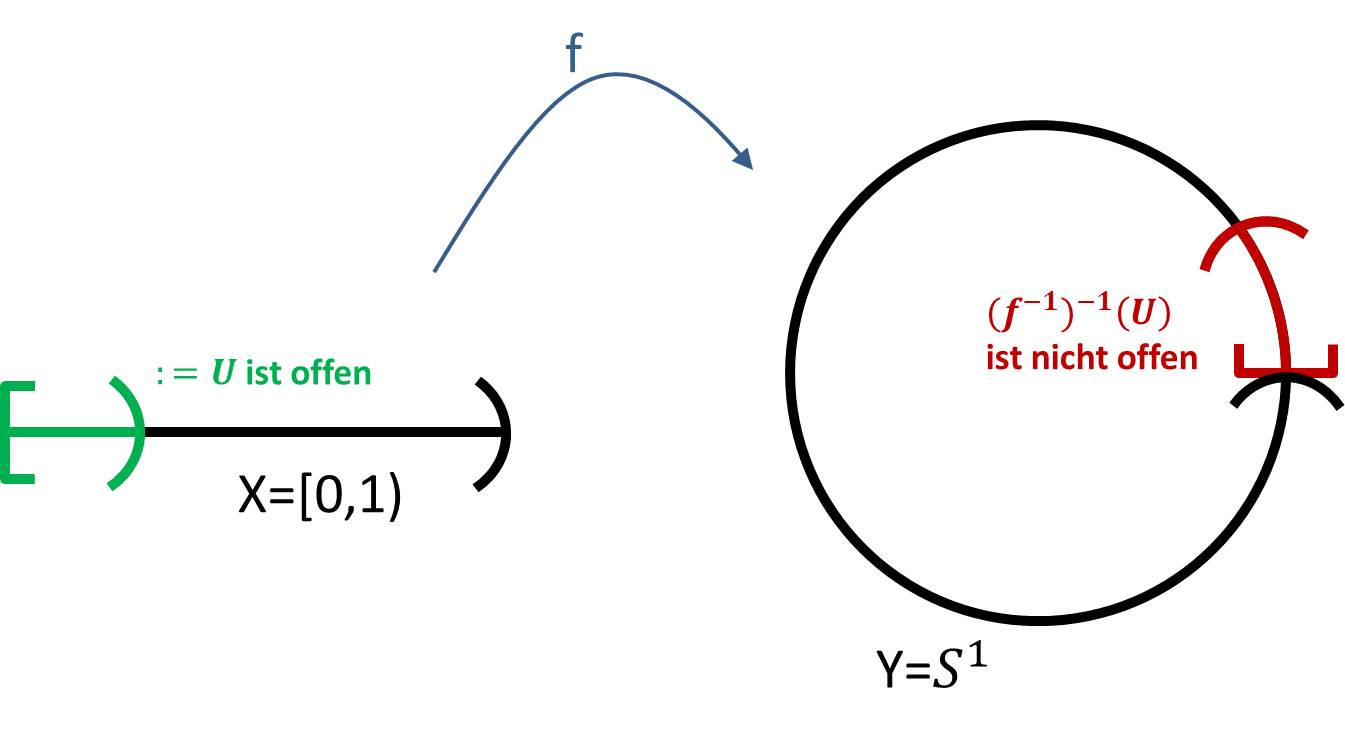
\includegraphics[width=0.75\textwidth]{images/0_1_nach_S1_f-1_nicht_stetig.jpg}}
\end{figure}

\section{Die Peano-Kurve}
(Guiseppe Peano, $\sim 1890$)
\begin{theorem}
	Es gibt eine surjektive, stetige Abbildung $I = [0,1] \rightarrow I \times I$.
\end{theorem}

\begin{figure}[h]
\centering
\subfloat[Iteration 1]{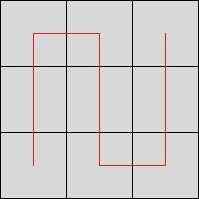
\includegraphics[width=0.4\textwidth]{images/PeanoKurve1.jpg}}\qquad
\subfloat[Iteration 2]{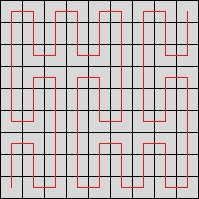
\includegraphics[width=0.4\textwidth]{images/PeanoKurve2.jpg}}
\caption{Prinzip der Peano-Kurve}
\end{figure}

\paragraph{Verallgemeinerung}
\begin{itemize}
\item Es gibt eine surjektive, stetige Abbildung $I \rightarrow I^n = I \times I \times \ldots \times I (n \in \N)$.
\item Es gibt eine surjektive, stetige Abbildung $\R \rightarrow \R^n$.
\end{itemize}

\subsection{Zugang mit Hilfe der Cantor-Menge $\mathcal{C}$}
Definiere $f \colon \mathcal{C} \rightarrow I, f \left(\sum\limits_{i=1}^{\infty}{\frac{a_i}{3}} \right) = \sum\limits_{i=1}^{\infty}{\frac{\frac{a_i}{2}}{2^i}}$ für $a_i \in \{0,2\}$.
\newline
Dann ist $f$ surjektiv und stetig.
\newline
Definiere $g \colon \mathcal{C} \rightarrow \mathcal{C} \times \mathcal{C}, g \left(\sum\limits_{i=1}^{\infty}{\frac{a_i}{3}} \right) = \left(\sum\limits_{i=1}^{\infty}{\frac{a_{2i}}{3^i}}, \frac{a_{2i+1}}{3^i} \right)=:(g_1,g_2)$ für $a_i \in \{0,2\}$.
\newline
Dann ist $g$ surjektiv und stetig.
\newline
Es ist auch $h \colon \mathcal{C} \rightarrow I \times I, x \mapsto \left(f(g_1(x)), f(g_2(x))\right)$ surjektiv und stetig.
\newline
Setze die Abbildung $h$ durch lineare Fortsetzungen stetig auf $I$ fort.

\chapter{07.11.2011}
\section{Nachträge und Wiederholungen zur Vorlesung}
\subsection{Überdeckung, Teilüberdeckung und Kompaktheit}
Sei $X$ ein topologischer Raum.
\begin{definition}
	\begin{itemize}
		\item Eine Familie $\{\mathcal{U}_\alpha \mid \alpha \in A \}$ von Teilmengen von $X$ heißt \underline{Überdeckung} von $X$, falls gilt: $X = \bigcup\limits_{\alpha \in A}{\mathcal{U}_\alpha}$.
		\item Eine Überdeckung heißt \underline{offen} (bzw. \underline{abgeschlossen}), falls alle $\mathcal{U}_\alpha (\alpha \in A)$ offen (bzw. abgeschlossen) sind.
		\item Es heißt $X$ \underline{kompakt}, falls jede offene Überdeckung $\mathcal{U}=\{U_\alpha, \alpha \in A\}$ eine endliche Teilüberdeckung $\mathcal{U}^\prime$ besitzt, d.h. es existiert $A^\prime \subset A$ endlich, so dass $\mathcal{U}^\prime = \{\mathcal{U}_\alpha \mid \alpha \in A^\prime \}$ eine offene Überdeckung von $X$ ist.
	\end{itemize}
\end{definition}

\begin{example}
	\begin{itemize}
		\item Endliche Räume und mit der trivialen Topologie versehene Räume sind kompakt.
		\item Diskrete Räume sind genau dann kompakt, wenn sie aus endlich vielen Elementen bestehen.
		\item $\R$ (versehen mit der Standardtopologie) ist \underline{nicht} kompakt, $\R_{\mathcal{T}_1}$ schon. ($\mathcal{T}_1 = \{ \R \backslash E \mid E \text{ endliche Teilmenge von } \R \} \cup \{\emptyset\}$)
	\end{itemize}
\end{example}

\begin{definition}	Eine \underline{kompakte Menge} ist eine Teilmenge eines vom Kontext her klaren topologischen Raumes, die bezüglich der Teilraumtopologie kompakt ist.
\end{definition}

\begin{example}
	$[0,1) (\subseteq \R)$ ist nicht kompakt, \underline{denn:} Die Überdeckung $\{(-1,1-\frac{1}{n}) \mid n \in \N \}$ von $[0,1)$ enthält keine endliche Teilüberdeckung.
\end{example}

\begin{remark}
	\begin{itemize}
		\item \underline{Satz von Heine-Borel:} Teilmengen euklidischer, endlich dimensionaler Räume sind genau dann kompakt, wenn sie abgeschlossen und beschränkt sind.
		\item Abgeschlossene Teilmengen kompakter Räume sind kompakt.
		\item Stetige Bilder kompakter Mengen sind kompakt, d.h. ist $X$ eine kompakte Menge, $Y$ topologischer Raum, $f \colon X \rightarrow Y$ stetig, dann ist $f(X)$ kompakt.
		\item Ist $X$ kompakt, $f \colon X \rightarrow \R$ stetig, so ist $f(X)$ kompakt und $f$ nimmt auf $X$ Maximum und Minimum an.
		\item \underline{Lebesque-Lemma:} Ist $f \colon X \rightarrow Y$ stetige Abbildung topologischer Räume und $X$ metrisch und kompakt, so gilt:
		\newline
			Ist $\mathcal{U}$ eine offene Überdeckung von $Y$, so existiert $\delta \in \R_{>0}$, sodass für alle $A \subseteq X$ mit diam $A < \delta$ ein $U^\prime \in \mathcal{U}$ mit $f(A) \subseteq U^\prime$ existiert.
	\end{itemize}
\end{remark}

\subsection{Wegzusammenhang}
\begin{definition}
	\begin{itemize}
		\item Ein \underline{Weg} in $X$ ist eine stetige Abbildung $\gamma \colon I(=[0,1]) \rightarrow X$ mit Anfangspunkt $\gamma(0)$ und Endpunkt $\gamma(1)$.	
		\item Man nennt $X$ \underline{wegzusammenhängend}, falls für alle $x,y \in X$ ein Weg $\gamma \colon [0,1] \rightarrow X$ in $X$ existiert mit $\gamma(0)=x, \gamma(1)=y$.
		\item Eine \underline{Wegzusammenhangskomponente} von $X$ ist eine wegzusammenhängende Teilmenge von $X$, die in keiner echt größeren solchen Teilmenge enthalten ist.
	\end{itemize}
\end{definition}

\begin{remark}
	\begin{itemize}
		\item Jeder Punkt von $X$ liegt in genau einer Wegzusammenhangskomponente von $X$, und zwei solche Komponenten sind entweder gleich oder disjunkt.
		\item Stetige Bilder wegzusammenhängender Mengen sind wegzusammenhängend.
	\end{itemize}
\end{remark}

\begin{corollary}
	Wegzusammenhang bleibt unter Homöomorphismen erhalten, ebenso die Anzahl der Wegzusammenhangskomponenten.
\end{corollary}

Wegzusammende topologische Räume sind zusammenhängend (Übungsaufgabe), die Umkehrung gilt im Allgemeinen nicht.

\paragraph{Beispiel eines Raumes, der zusammenhängend, aber nicht wegzusammenhängend ist}
Definiere $A = \{(x,y) \in \R^2 \mid x > 0, y = \sin{\left(\frac{1}{x}\right)}\}, X := A \cup \{(0,0)\}$.
\newline
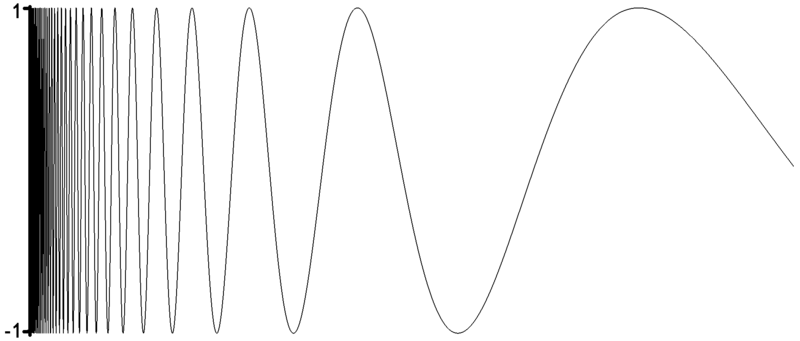
\includegraphics[scale=0.4]{images/Sinuseinsdurchx.png}
\newline
Es gilt:
\begin{itemize}
	\item Es ist $A$ wegzusammenhängend, denn:
	 \newline	
	 $A \cong (0, +\infty) \cong \R$, und $\R$ ist wegzusammenhängend.
	\item Es ist $X$ zusammenhängend, denn:
		\newline
		Es gilt: $\bar{A} = A \cup \{(0,y) \mid y \in [-1,1]\}$ ist als Abschluss einer zusammenhängenden Menge wieder zusammenhängend (siehe Bemerkung in der Vorlesung).
		\newline
		Außerdem gilt: $A \subseteq X \subseteq \bar{A}$, und $X$ ist als Teilmenge des Abschlusses eines zusammenhängenden Raumes wieder zusammenhängend. (\underline{Allgemein:} Es sei $A$ zusammenhängend, $A \subseteq B \subseteq \bar{A}$. Dann ist auch $B$ zusammenhängend.)
	\item Es ist $X$ \underline{nicht wegzusammenhängend}, denn:
		\newline
		Es lässt sich $(0,0)$ nicht über einen Weg in $X$ mit einem beliebigen anderen Punkt aus $X$ verbinden\footnote{Formale Begründung: Jeder in $(0,0)$ startende Weg ist konstant.}.
\end{itemize}

\begin{remark}
	Der Abschluss wegzusammenhängender Räume ist im Allgemeinen nicht wegzusammenhängend!
\end{remark}

\begin{example}[Beispiel von oben]
	Der Abschluss von $A$ \underline{in $X$} - nicht in $\R^2$ - ist $X$, und $X$ ist (s.o.) nicht wegzusammenhängend.
\end{example}

\begin{remark}
	Besitzt jeder Punkt eines topologischen Raumes $X$ eine wegzusammenhängende Umgebung, so sind alle Wegzusammenhangskomponenten offen in $X$, und $X$ ist genau dann wegzusammenhängend, wenn $X$ zusammenhängend ist.
\end{remark}

\begin{example}
	Offene Teilmengen von $\R^n$ sind genau dann wegzusammenhängend, wenn sie zusammenhängend sind, \underline{denn:}
	\newline
	Jeder Punkt $x \in \R^n$ besitzt dann als offene Umgebung einen offenen Ball, und offene Bälle sind wegzusammenhängend.
\end{example}

\chapter{14.11.2011}
\section{Beispiele für Beweise im Kontext von Hausdorffräumen}
\begin{theorem}{Behauptung:}
Ist $X$ ein Hausdorffraum, so besitzt jede Folge $(x_n)_{n \in \N} \in X^\N$ höchstens einen Grenzwert.
\end{theorem}
\begin{proof}
	Sei $X$ ein Hausdorffraum.
	\newline
	\underline{Annahme:} Es existiert eine Folge $(x_n)_{n \in \N} \in X^\N$ mit $x = \lim\limits_{n \rightarrow \infty}(x_n) = x^\prime$ und $x \neq x^\prime$.
	\newline
	Da $X$ Hausdorffsch ist, existieren offene Teilmengen $U,V \subseteq X$, mit $U \cap V = \emptyset$ und $x \in U, x^\prime \in V$. Dann existieren $n_0, n_0^\prime \in \N$ mit $x_n \in U, x_m \in V \text{ für alle } n \in \N_{\geq n_0}, m \in \N_{\geq n_0^\prime}$. Dann gilt also für alle $k \geq \max\{n_0,n_0^\prime\} \colon x_k \in U \cap V=\emptyset$. $\lightning$
\end{proof}

\begin{theorem}
Jeder metrische Raum ist Hausdorffsch.
\end{theorem}

\begin{proof}
[\underline{z.z.:} $\forall x\neq y \in X \exists U_x, U_y \subseteq X \colon U_x \cap U_y = \emptyset$.]
Seien $x\neq y \in X$. Wähle $U_x := B_\frac{d(x,y)}{3}(x), U_y := B_\frac{d(x,y)}{3}(y)$.
\newline
Dann gilt: $U_x \cap U_y = \emptyset$.
\end{proof}

\section{Beispiele für Mannigfaltigkeiten}
\begin{enumerate}
	\item Was sind 0-dimensionale Mannigfaltigkeiten?
		\begin{itemize}
			\item Abzählbare diskrete Mengen.
		\end{itemize}
		
	\item \underline{1-dimensionale glatte Mannigfaltigkeiten} \newline
	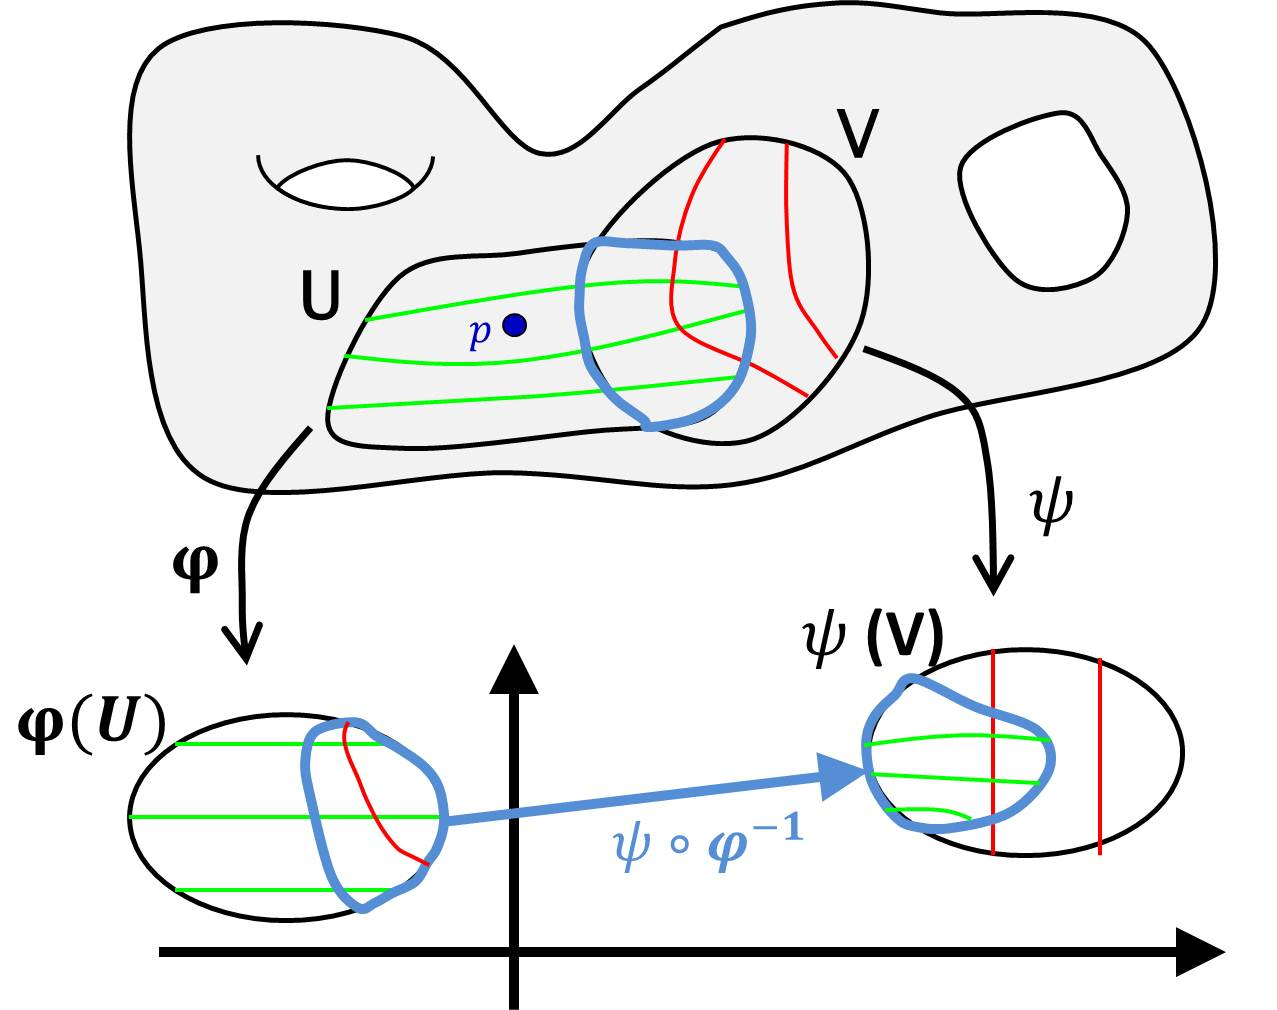
\includegraphics[scale=0.4]{images/Kartenwechsel.jpg}
		\begin{itemize}
			\item Offene Intervalle in $\R$ sind 1-dimensionale glatte Mannigfaltigkeiten, \underline{denn:} Seien $a,b \in \R$ mit $a < b$.
			\begin{itemize}
				\item $(a,b)$ ist als metrischer Raum Hausdorffsch.
				\item Es ist $\mathcal{B} = \{B_{\frac{1}{n}}(x) \mid x \in \Q, n \in \N\}$ eine abzählbare Basis der Topologie.
				\item $(a,b)$ ist lokal homöomorph zu $\R$, \underline{denn:} Es gilt: $id \colon (a,b) \mapsto (a,b) \subseteq \R$ ist ein Homöomorphismus einer offenen Menge in eine offene Teilmenge von $\R$. Somit ist $\left((a,b),id_{(a,b)}\right)$ eine (\underline{globale})\footnote{Global, da für die ganze Mannigfaltigkeit gleich.} Karte.
				\item Für den Kartenwechsel gilt: $id_{(a,b)} \circ id_{(a,b)}^{-1} \colon (a,b) \rightarrow (a,b), x \mapsto x$, ist eine glatte Abbildung.
			\end{itemize}
		
		\item $S^1 = \{ x \in \R^2 \mid ||x|| = 1\}$ \newline
		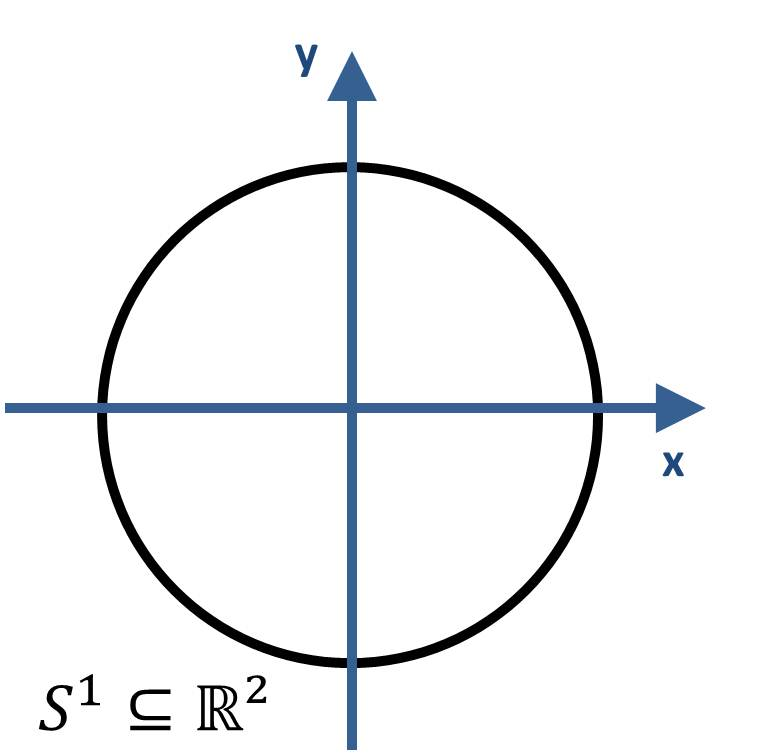
\includegraphics[scale=0.4]{images/S1.jpg} \newline
		ist eine 1-dimensionale glatte Mannigfaltigkeit, \underline{denn:}
			\begin{itemize}
				\item Es ist $S^1$ als Teilmenge des metrischen Raumes $\R^2$ Hausdorffsch.
					\newline
					Ebenso besitzt $S^1$ eine abzählbare Basis der Topologie.
				\item Definiere $$U_1 := \{(x,y) \in S^1 \mid y \neq 1\} = S^1 \backslash \{N\} \quad \left(N := (0,1)\right)$$ und $$U_2 := \{(x,y) \in S^1 \mid y \neq -1\} = S^1 \backslash \{S\} \quad \left(S := (0,-1)\right).$$
				Dann gilt:
				\item $U_1 \cup U_2 = S^1$,
				\item Es sind $U_1$ und $U_2$ offene Teilmengen von $S^1$, denn sie sind jeweils Komplement einer einpunktigen und damit abgeschlossenen Menge.
				\item Definiere $$\varphi_1 \colon U_1 \rightarrow \R, (x,y) \mapsto \frac{x}{1-y},$$
				$$\varphi_2 \colon U_2 \rightarrow \R, (x,y) \mapsto \frac{x}{1+y}.$$
				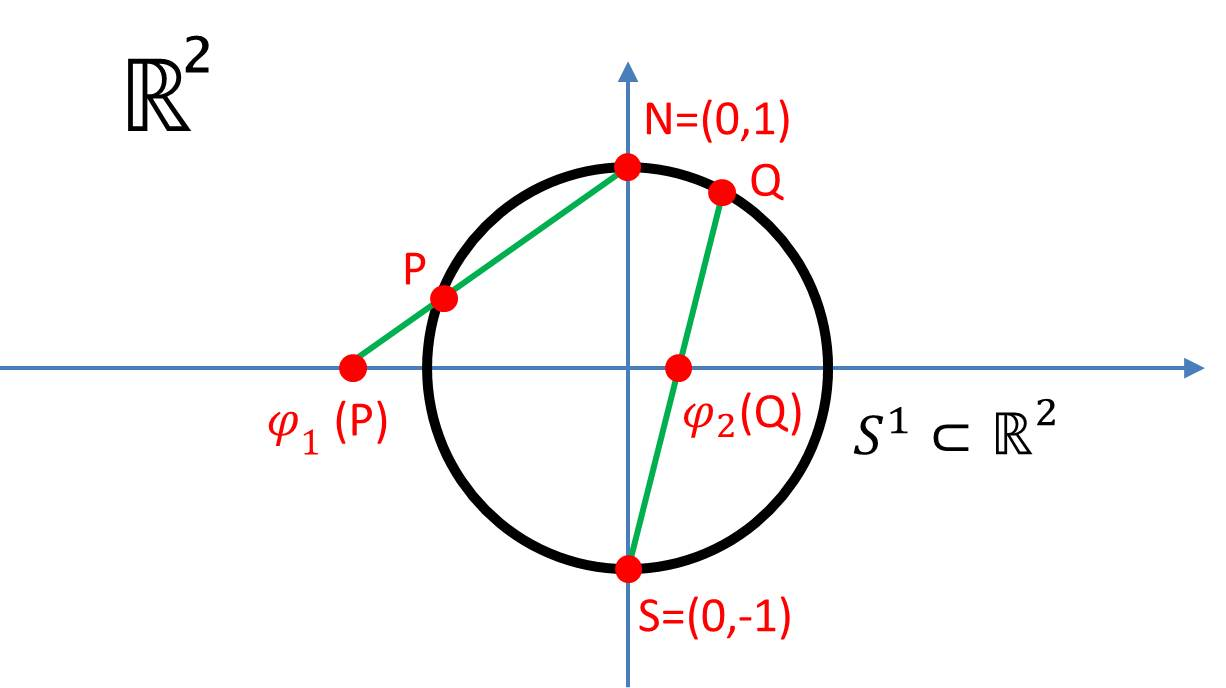
\includegraphics[scale=0.4]{images/Stereographie.jpg} \newline
				Im Folgenden zeigen wir, dass $(U_1, \varphi_1)$ eine Karte ist. Analoges gilt auch für $(U_2, \varphi_2)$ mit analoger Rechnung.
				\item Definiere $$\psi \colon \R \rightarrow S^1, u \mapsto (\frac{2u}{u^2+1}, \frac{u^2-1}{u^2+1}).$$
				Dann gilt:
				$$\varphi_1 \circ \psi = id_\R,$$
				$$\psi \circ \varphi_1 = id_{U_1}.$$
				Damit ist $\varphi_1$ bijektiv.
				\newline
				Da $\varphi_1$ und $\psi$ stetig sind, ist $\varphi_1$ damit ein Homöomorphismus.
				\item Die Kartenwechsel sind glatt, denn es gilt:
				$$\varphi_1(U_1 \cap U_2) = \R \backslash \{0\} = \varphi_2(U_1 \cap U_2).$$
				Für alle $u \in \R \backslash \{0\}$ gilt:
				$$(\varphi_2 \circ \varphi_1^{-1})(u) = (\varphi_2 \circ \psi)(u) = \frac{1}{u},$$
				und dies ist tatsächlich ein $C^\infty-$Diffeomorphismus\footnote{d.h. bijektiv und unendlich oft differenzierbar und mit unendlich oft differenzierbarer Umkehrabbildung} $\R \backslash \{0\} \rightarrow \R \backslash \{0\}$.
			\end{itemize}
	\end{itemize}			
	
	\item Es ist $\R^n$ eine $n$-dimensionale glatte Mannigfaltigkeit, \underline{denn:}
		\begin{itemize}
			\item $\R^n$ ist Hausdorffsch und besitzt eine abzählbare Basis der Topologie.
			\item $(\R^n, id_{\R^n})$ ist eine globale Karte.
		\end{itemize}
\end{enumerate}

\begin{remark}
	Jeder Atlas, der aus nur einer Karte besteht, ist glatt.
\end{remark}

\begin{proof}
	Es sei $\mathcal{A} = \{(\varphi,U)\}$ dieser Atlas. Dann gilt:
	\newline
	Es gibt nur genau einen Kartenwechsel: 
	$$\varphi \circ \varphi^{-1} = id_{\varphi(U)} \colon \varphi(U) \rightarrow \varphi(U)$$ und dieser ist natürlich glatt.
\end{proof}

\begin{theorem}
	Offene Teilmengen von $C^k$-Mannigfaltigkeiten sind wieder $C^k$-Mannigfaltigkeiten.
\end{theorem}

\begin{proof}
	Es sei $M$ eine $C^k$-Mannigfaltigkeit der Dimension $n$, $N \subseteq_{offen} M$.
	\begin{itemize}
		\item Als Teilmenge von $M$ ist $N$ Hausdorffsch und auch die abzählbare Basis der Topologie überträgt sich.
		\item Es sei $\mathcal{A} = \{(\varphi_\alpha, U_\alpha) \mid \alpha \in \Lambda \}$ ($\Lambda$ Indexmenge) ein $C^k$-Atlas von $M$.
		\newline
		Für alle $\alpha \in \Lambda$ ist $U_k \cap N$ offen in $N$ und es gilt:
		$$\varphi_\alpha \big |_{U_\alpha \cap N} \colon U_\alpha \cap N \rightarrow \varphi_\alpha(U_\alpha \cap N) \subseteq \R^n$$
		und $\varphi_\alpha(U_\alpha \cap N)$ ist als stetiges Bild der offenen Menge $U_\alpha \cap N$ wieder offen.
		\newline
		Somit ist $\{(\varphi_\alpha \big |_{U_\alpha \cap N}, U_\alpha \cap N) \mid \alpha \in \Lambda\}$ ein Atlas für $N$.
		\newline
		Da die Kartenwechsel weiterhin $C^k$-Abbildungen sind, ist dieser Atlas ein $C^k$-Atlas für $N$.
	\end{itemize}
\end{proof}

\begin{example}
	Es gilt: $GL(n,\R) = \det^{-1}(\R \backslash \{0\}) \subseteq_{offen} \R^{n^2}$
\end{example}

\chapter{21.11.11}

\section{Untermannigfaltigkeiten}
\begin{theorem}{$C^\infty$-Untermannigfaltigkeiten von $\R^{n+l}$ sind $C^\infty$-Mannigfaltigkeiten}
	Es sei $M \subseteq \R^{n+l}$ eine $n$-dimensionale $C^\infty$-Untermannigfaltigkeit von $\R^{n+l}$, versehen mit der Teilraumtopologie, und $\{\psi_\alpha \colon W_\alpha \rightarrow U_\alpha \cap M\ \mid \alpha \in \Lambda\}$ eine Menge lokaler Parametrisierungen (siehe Untermannigfaltigkeitskriterium, (c)) mit $M \subseteq \bigcup\limits_{\alpha \in \Lambda}{U_\alpha}$.
	\newline
	Dann ist $\mathcal{A}=\{(\psi_\alpha^{-1}, U_\alpha \cap M) \mid \alpha \in \Lambda\}$ ein $C^\infty$-Atlas für $M$ und $M$ somit eine $C^\infty$-Mannigfaltigkeit.
\end{theorem}

\begin{proof}
	\begin{itemize}
		\item Es gilt: $M$ ist Hausdorffsch und besitzt eine abzählbare Basis der Topologie (als Teilmenge von $\R^{n+l}$).
		\item Es ist $\mathcal{A}$ ein Atlas (nach Definition der lokalen Parametrisierungen).
		\item $[$\underline{z.z.:} Die Kartenwechsel sind glatt, d.h.: 
			$$\forall \alpha, \beta \in \Lambda \colon (U_\alpha \cap M) \cap (U_\beta \cap M) \neq \emptyset$$
			$$\Rightarrow \psi_\beta^{-1} \circ \psi_\alpha \colon \psi_\alpha^{-1}(U_\alpha \cap U_\beta \cap M) \rightarrow \psi_\beta(U_\alpha \cap U_\beta \cap M)$$
			 ist glatt.$]$ \newline
			Seien $\alpha, \beta \in \Lambda$ mit $(U_\alpha \cap M) \cap (U_\beta \cap M) \neq \emptyset$.
			\newline
			(\underline{Vorsicht:} Es ist $\psi_\beta^{-1}$ nicht auf einer offenen Teilmenge von $\R^{n+l}$ definiert, daher ist die Kettenregel nicht direkt anwendbar!)
			\newline
			\underline{Zeige:} Es ist $\psi_\beta^{-1}$ auf einer (offenen) Umgebung eines jeden Punktes $y \in U_\alpha \cap U_\beta \cap M$ eine glatte Abbildung.
			\newline
			Sei $x \in \psi_\alpha^{-1}(U_\alpha \cap U_\beta \cap M)$. Nach dem Untermannigfaltigkeits-Kriterium (b) existiert eine Umgebung $U \subseteq U_\alpha \cap U_\beta$ von $\psi_\alpha(x) \in M$ in $\R^{n+l}$ und ein $C^\infty$-Diffeomorphismus $\varphi \colon U \rightarrow \varphi(U) \subseteq \R^{n+l}$ mit $\varphi(U \cap M) = \varphi(U) \cap (\R^{n} \times \{0\})$
			\newline
			Definiere $\pi \colon \R^{n+l} \cong \R^n \times \R^l \rightarrow \R^n$, die Projektion auf die ersten $n$ Komponenten und $\iota \colon \R^n \hookrightarrow \R^{n+l}, x \mapsto (x,0)$, die Inklusion. Dann gilt auf $\varphi(U \cap M) \subseteq \R^{n} \times \{0\}$: $\iota \circ \pi = id$. Daher gilt auf $\psi_\alpha^{-1}(U \cap M)$: 
			$$\psi_\beta^{-1} \circ \psi_\alpha = \psi_\beta^{-1} \circ \varphi^{-1} \circ \varphi \circ \psi_\alpha = (\psi_\beta^{-1} \circ \varphi^{-1} \circ \iota)\circ(\pi \circ \varphi \circ \psi_\alpha).$$
			Es sind $(\psi_\beta^{-1} \circ \varphi^{-1} \circ \iota) = (\pi \circ \varphi \circ \psi_\beta)^{-1}$ und $\pi \circ \varphi \circ \psi_\alpha$ glatte Abbildungen zwischen offenen Teilmengen des $\R^n$ und somit auch die Komposition $\psi_\beta^{-1} \circ \psi_\alpha$.
	\end{itemize}
\end{proof}

\section{Wichtige Spezialfälle (und Beispiele) von Untermannigfaltigkeiten}
\paragraph{(a) Niveaumengen}
Es seien $V \subseteq \R^{n+l}$ offen, $f \in C^\infty(V,\R^l)$ und $c \in \R^l$. Gilt Rang $Df(x)=l$ in jedem Punkt $x$ der Niveaumenge
$$f^{-1}(c) := f^{-1}(\{c\}) = \{x \in V \mid f(x) = c\},$$
so ist $f^{-1}(c)$ eine $n$-dimensionale glatte Untermannigfaltigkeit von $\R^{n+l}$.

\begin{proof}
	Wende Untermannigfaltigkeits-Kriterium (a) auf die Abbildung $$g = f - c \colon x \mapsto f(x)-c$$ an.
	\newline
	$[$\underline{z.z.:} Rang $Df(x)=l$ auf einer Umgebung $U$ von $f^{-1}(c)$, nicht nur auf der Niveaumenge selbst!$]$
	\newline
	Sei $x_0 \in f^{-1}(c)$. Da Rang $Df(x_0) = l$, existiert eine $(l \times l)$-Unterdeterminante $A(x)$ von $\det{Df(x)}$, so dass $A(x_0)\neq 0$. Da $f$ stetig ist, ist die Abbildung $x \mapsto A(x)$ stetig, und somit folgt: $A(x)\neq 0$ auf einer Umgebung $U(x_0)$ von $x_0$. Dann ist Rang $Df(x)=l$ für alle $x \in U(x_0)$.
	\newline
	Setze $U:= \bigcup\limits_{x_0 \in f^{-1}(c)}{U(x_0)}$, dann folgt die Behauptung.
\end{proof}

\begin{example}
	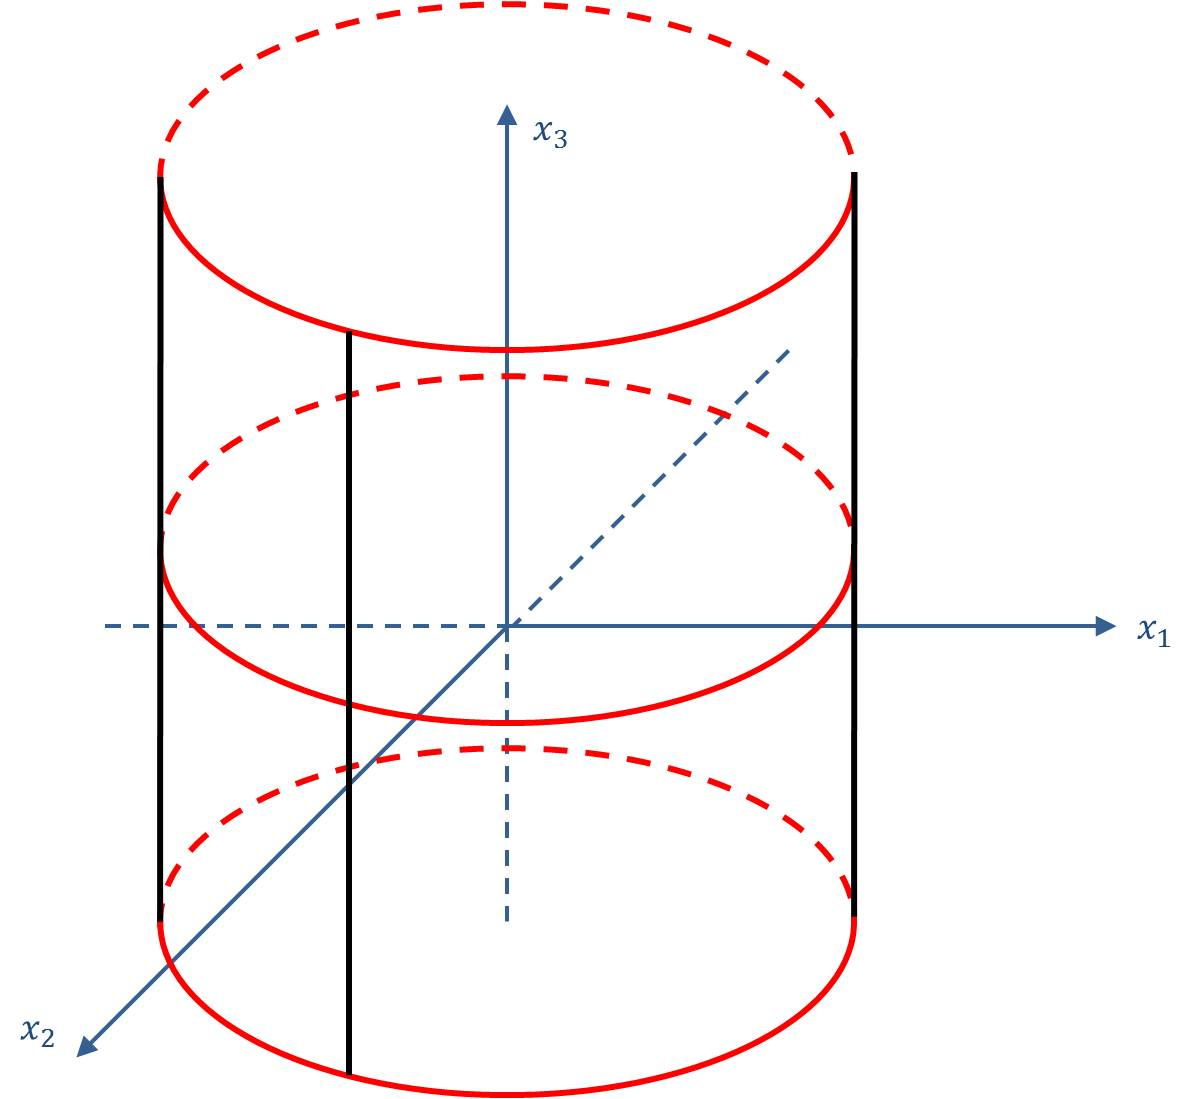
\includegraphics[scale=0.4]{images/Zylinder.jpg}
	\newline
	Der \underline{Zylinder} $M=\{(x,y,z) \in \R^3 \mid x^2+y^2 = 1\}$ ist als Niveaumenge der Abbildung $f \colon \R^3 \rightarrow \R, (x,y,z) \mapsto \underbrace{x^2+y^2}-1$, eine $C^\infty$-Untermannigfaltigkeit von $\R^3$.
\end{example}

\paragraph{(b)}
\begin{example}
	Der Graph der Abbildung $\varphi \colon \R \rightarrow \R^2, t \mapsto (\cos{(t)},\sin{(t)})$, d.h. die Menge $\{(\cos{(t)},\sin{(t)},t) \mid t \in \R\}$, die \underline{Helix},
\begin{figure}[h]
	\centering
	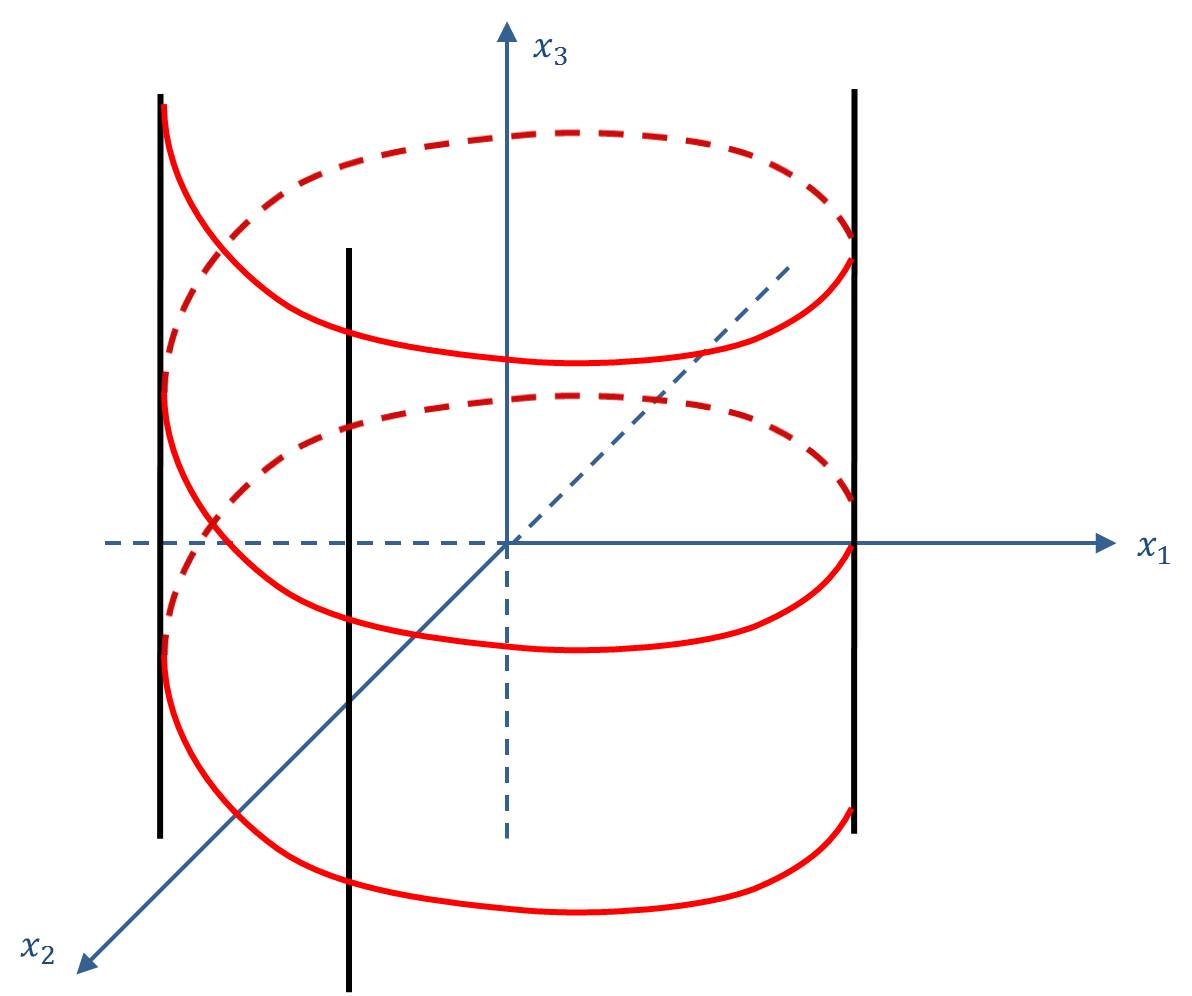
\includegraphics[scale=0.4]{images/Helix.jpg}
\end{figure}
 ist eine 1-dimensionale glatte Untermannigfaltigkeit von $\R^3$.
\end{example}

\paragraph{(c) Global parametrisierte Untermannigfaltigkeiten}
Es sei $W \subseteq \R^n$ offen und $\psi \colon W \rightarrow \R^{n+l}$ glatt mit Rang $D\psi(w)=n$ für alle $w \in W$. Es sei ferner $\psi \colon W \rightarrow \psi(W)$ Homöomorphismus.
Dann ist $\psi(W)$ eine $C^\infty$-Untermannigfaltigkeit von $\R^{n+l}$ (nach Untermannigfaltigkeits-Kriterium (c) mit $U := \R^{n+l}$).
\newline
Für $n=2$ und $l=1$ heißt $\psi(W)$ eine \underline{parametrisierte Fläche} von $\R^3$.

\begin{example}
	\begin{enumerate}
		\item Parametrisierung des Zylinders:
			\newline
			Betrachte die glatte Abbildung $\psi \colon (0, 2 \pi) \times \R \rightarrow \R^3, (t,s) \mapsto (\cos{(t)}, \sin{(t)}, s)$. Das Bild dieser Abbildung ist der Zylinder im $\R^3$ (wie oben, ohne eine Gerade).
			Es gilt:
			$$D\psi(t,s) = \begin{pmatrix} -\sin{(t)} & 0 \\ \cos{(t)} & 0 \\ 0 & 1  \end{pmatrix} $$ für alle $(t,s) \in \R^2$, und damit:
			Rang $D \psi(t,s)=2$ für alle $(t,s) \in \R$, da $\sin$ und $\cos$ keine gemeinsamen Nullstellen haben.
			\newline
			Damit ist $\psi$ eine (globale) Parametrisierung des Zylinders.
			
		\item (Rotationsflächen im $\R^3$)
			\newline
			Rotiere für Konstanten $0 < r < a$ die Kurve $\gamma \colon [0,2\pi] \rightarrow \R^3, t \mapsto (a + r \cdot \cos{(t)}, 0, r \cdot \sin{(t)})$.
			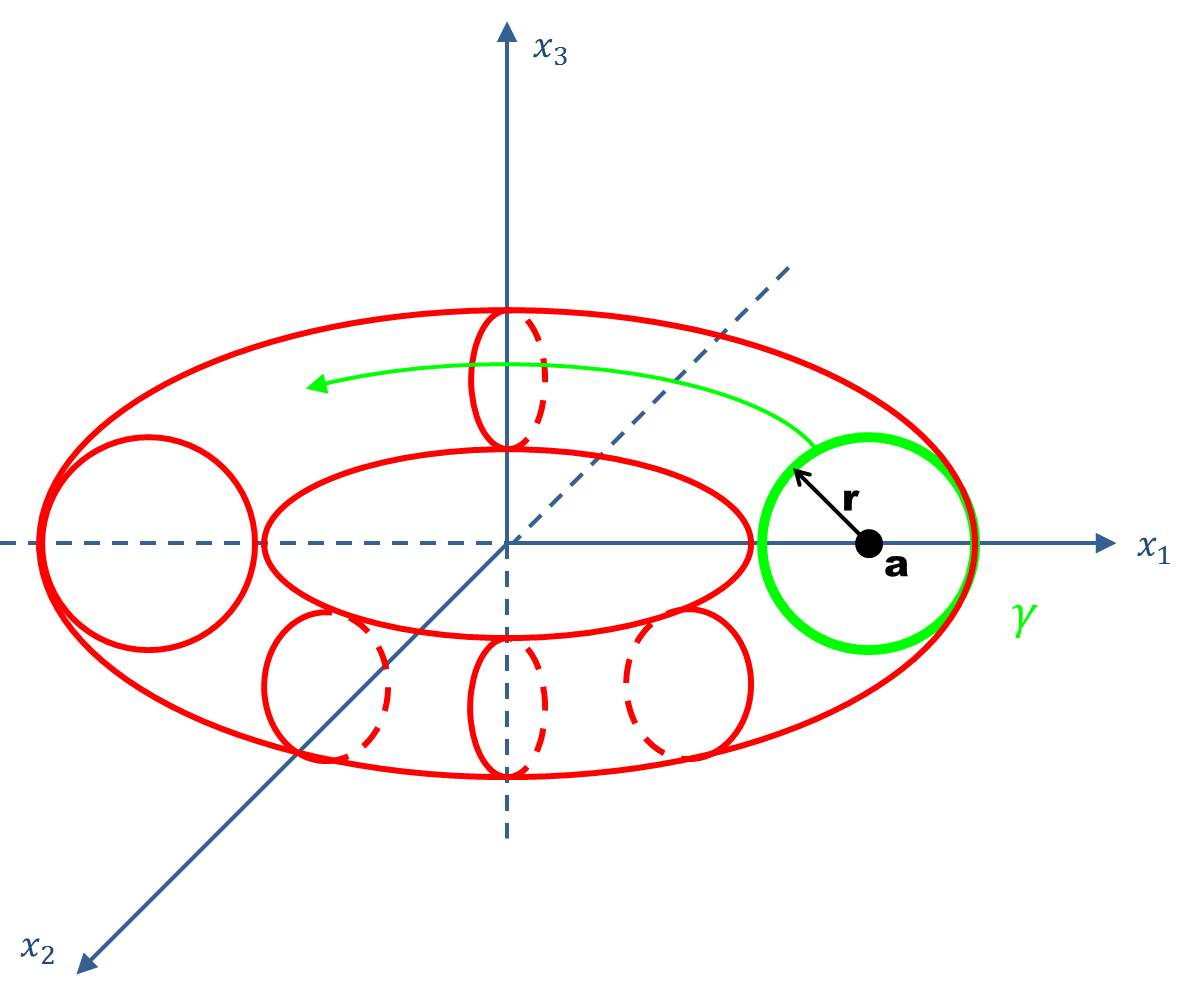
\includegraphics[scale=0.4]{images/Torus_Rotation.jpg} in der $x_1 x_3$-Ebene:
			$$\begin{pmatrix}
				x \\ y \\z
			\end{pmatrix} = \begin{pmatrix}
			\cos{\Theta} & -\sin{\Theta} & 0 \\ \sin{\Theta} & \cos{\Theta} & 0 \\ 0 & 0 & 1
\end{pmatrix} \begin{pmatrix}
	a + r \cdot \cos{(t)} \\ 0 \\ r \cdot \sin{(t)}
\end{pmatrix}$$

	$$= \underbrace{\begin{pmatrix}
	(a + r \cdot \cos{(t)})  \cos{(\Theta)} \\ (a + r \cdot \cos{(t)})  \sin{(\Theta)} \\ r \cdot \sin{(t)}
	\end{pmatrix} }_{(*)}$$
	Dann definiert $\Phi_\gamma \colon (0, 2\pi) \times (0, 2 \pi) \rightarrow \R^3, (\Theta, t) \mapsto (*)$
	eine parametrisierte Fläche, den Rotationstorus.
	\newline
	$\bullet$ Der Rotationstorus $T \subseteq \R^3$ lässt sich als Niveaumnge definieren: 
	$$T = \{(x,y,z) \in \R^3 \mid z^2 + (\sqrt{x^2+y^2}-a)^2 = r^2\}.$$
	$\bullet$ Eine weitere (aus der Vorlesung bekannte) Darstellung des Torus ist
	$$S^1 \times S^1 = \{(x_1,x_2,x_3,x_4) \in \R^4 \mid (x_1)^2 + (x_2)^2 = 1 \wedge (x_3)^2 + (x_4)^2 = 1 \},$$
	und dies ist nicht die letzte Möglichkeit der Darstellung des Torus (siehe nächste Vorlesung) \ldots 
	\end{enumerate}
\end{example}

\chapter{05.12.2011}
\section{Homotopieäquivalenzen}
\paragraph{Definition}
Für zwei topologische Räume $X,Y$ heißt eine $\underbrace{\text{stetige Abbildung }f \colon X \rightarrow Y}_{f \in C(X,Y)}$ \textbf{Homotopieäquivalenz}, falls es eine stetige Abbildung $g \colon Y \rightarrow X$ gibt, sodass $g \circ f \simeq id_x$ und $f \circ g \simeq id_Y$ gilt.

\begin{proposition}
	Es seien $X,Y$ topologische Räume. Die Relation "$\simeq$" ist eine Äquivalenzrelation auf $C(X,Y)$.
\end{proposition}

\begin{proof}
	\begin{itemize}
		\item Reflexivität: Es sei $f \in C(X,Y)$.
			Definiere $H \colon X \times I \rightarrow Y, (x,t) \mapsto f(x)$.
			Dann ist $H$ eine Homotopie von $f$ nach $f$, was die Reflexivität von "$\simeq$" zeigt.
		\item Symmetrie: Es seien $f,g \in C(X,Y)$ mit $f \simeq g$, d.h. es existiert eine Homotopie $H$ von $f$ nach $g$. Definiere $G \colon X \times I \rightarrow Y, (x,t) \mapsto H(x,1-t)$.
		Dann ist $G$ Homotopie von $g$ nach $f$ und die Symmetrie von "$\simeq$" gezeigt.
		\item Transitivität: Es seien $f,g,h \in C(X,Y)$ mit $f \simeq g \simeq h$ durch die Homotopien $H_1$ und $H_2$. Definiere 
			$$H \colon X \times I \rightarrow Y, (x,t) \mapsto \begin{cases} H_1(x,2t),& 0 \leq t \leq \frac{1}{2} \\ H_2(x,2t-1), & \frac{1}{2} \leq t \leq 1 \end{cases}$$
			Dann gilt für alle $x \in X$:
			\begin{itemize}
				\item $H(x,0) = H_1(x,0)=f(x),$
				\item $H(x,1) = H_2(x,1)=h(x),$
			\end{itemize}
			Für $t = \frac{1}{2}$ betrachte:
			$$\lim\limits_{t \nearrow \frac{1}{2}}{H(x,t)} = \lim\limits_{t \nearrow \frac{1}{2}}{H_1(x,2t)} = H_1(x,1) = g(x),$$
			$$\lim\limits_{t \searrow \frac{1}{2}}{H(x,t)} = \lim\limits_{t \searrow \frac{1}{2}}{H_2(x,2t-1)}=H_2(x,0)=g(x).$$
			Damit ist $H$ Homotopie von $f$ nach $h$ und die Transitivität von "$\simeq$" gezeigt.
	\end{itemize}
\end{proof}

\section{Beispiele zu Homotopien}
\begin{enumerate}
	\item \underline{Beh.:} Für einen topologischen Raum $X$ sind je zwei Abbildungen $f,g \colon X \rightarrow \R^n$ \footnote{\underline{Statt $\R^n$ reicht:} kontrahierbarer Raum} homotop.
	\begin{proof}
		Sei $X$ ein topologischer Raum, $f,g \in C(X,\R^n)$.
		Definiere $H \colon X \times I \rightarrow \R^n, (x,t) \mapsto (1-t)f(x) + t \cdot g(x)$.
		Dann ist $H$ Homotopie von $f$ nach $g$, eine \textbf{lineare} Homotopie.
	\end{proof}
	
	\item \underline{Beh.:} Jede stetige Abbildung $\R^n \rightarrow Y, Y$ topologischer Raum, ist nullhomotop.
	\begin{proof}
		Es sei $Y$ topologischer Raum $f \in C(\R^n,Y)$.
		Definiere $H \colon \R^n \times I \rightarrow Y, (x,t) \mapsto f((1-t)x).$
		Dann gilt für alle $x \in \R^n:$
		\begin{itemize}
			\item $H(x,0)=f((1-0)x) = f(x),$
			\item $H(x,1)=f((1-1)x) = f(0).$
		\end{itemize}
		Dann ist $H$ Homotopie $f$ nach $c_{f(0)} (=c \equiv f(0)).$
	\end{proof}
\end{enumerate}

\paragraph{Definition:} Es seien $X,Y$ topologische Räume, $A \subseteq X$. Seien $f,g \in C(X,Y).$
Es heißt \underline{$f$ relativ $A$ homotop zu $g$} (in Zeichen $f \simeq g \text{ rel } A$), falls eine Homotopie $H \colon X \times I \rightarrow Y$ von $f$ nach $g$ existiert, so dass $H(a,t)=H(a,0)$ für alle $a \in A, t \in I$.

\begin{remark}{} Es seien $X,Y$ topologische Räume, $A \subseteq X$. Dann ist "Homotopie rel $A$" eine Äquivalenzrelation.
\end{remark}

\begin{proposition} Homotopieäquivalenz ist eine Äquivalenzrelation (auf der Klasse der topologischen Räume).
\end{proposition}

\begin{remark}
	$ $
	\begin{itemize}
		\item Reflexivität: Es sei $X$ topologischer Raum.
			Es gilt: $X \simeq X$ durch die Homotopieäquivalenz $\tilde{f},\tilde{g} := id_X$.
		\item Symmetrie: Seien $X,Y$ topologische Räume mit $X \simeq Y$, d.h. es existieren $\tilde{f} \in C(X,Y), \tilde{g} \in C(Y,X)$ mit $\tilde{g} \circ \tilde{f} \simeq id_X, \tilde{f} \circ \tilde{g} \simeq id_Y$.
		Definiere $f:= \tilde{g}, g:= \tilde{f}$.
		Dann gilt $f \circ g \simeq id_X, g \circ f \simeq id_Y,\text{ d.h. }Y \simeq X.$
		
		\item Transitivität: Seien $X,Y,Z$ topologische Räume mit $X \simeq Y \simeq Z$, d.h. es existieren $f_1 \in C(X,Y), g_1 \in C(Y,X), f_2 \in C(Y,Z), g_2 \in C(Z,Y)$ mit
		$$g_1 \circ f_1 \simeq id_X, f_1 \circ g_1 \simeq id_Y$$
		$$g_2 \circ f_2 \simeq id_Y, f_2 \circ g_2 \simeq id_Z$$
		Definiere $f := f_2 \circ f_1, g:= g_1 \circ g_2$. Dann gilt:
		$$g \circ f \simeq id_X, f \circ g \simeq id_Z,$$
		d.h. $X \simeq Z$.
	\end{itemize}
\end{remark}

\section{Kontrahierbarkeit}
Es sei $X$ ein topologischer Raum.

\paragraph{Definition} Man nennt $X$ \textbf{kontrahierbar}, falls gilt: $X \simeq \{pt\}$.

\begin{remark}
	Es gilt:
	$$X \text{ kontrahierbar } \Leftrightarrow id_X \text{ ist nullhomotop.}$$
\end{remark}

\begin{example}{}
$ $
\begin{itemize}
	\item Es ist $\R^n$ kontrahierbar, \underline{denn}: \newline
	Definiere $H \colon \R^n \times I \rightarrow \R^n, (x,t) \mapsto (1-t)x$.
	Dann ist $H$ Homotopie von $id_X$ nach $c_0$, d.h. $\R^n$ ist kontrahierbar nach obiger Bemerkung.
	\item Genauer ist jede \textbf{sternförmige}\footnote{Es existiert $x_0 \in M$, so dass für alle $x \in M$ gilt: $(1-t)x + t \cdot x_0 \in M$} 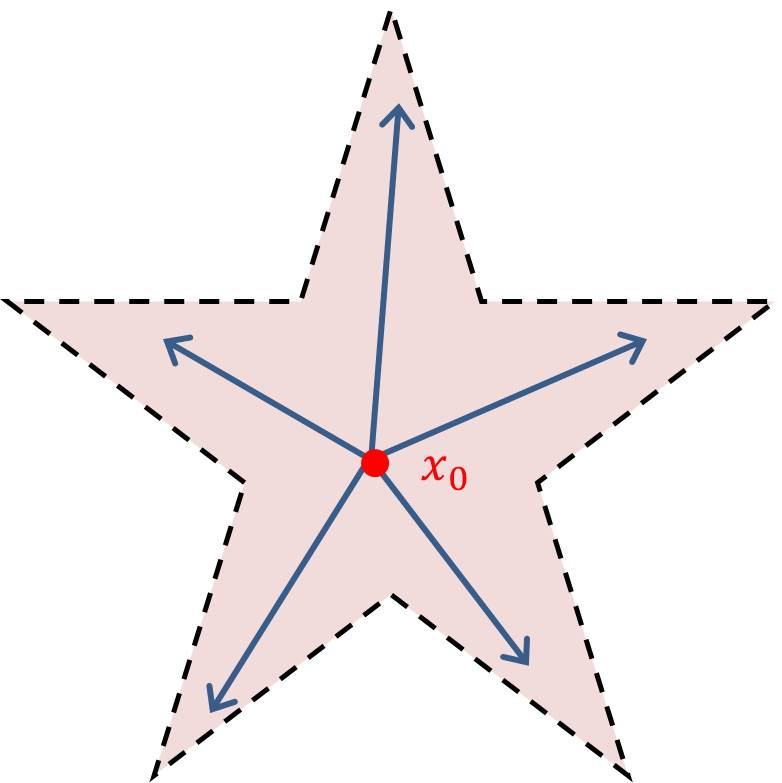
\includegraphics[scale=0.3]{images/sternfoermig.jpg} Teilmenge $M \subseteq \R^n$ kontrahierbar.
		\begin{example}
			$D^n, B^n$.
		\end{example}
\end{itemize}
\end{example}

\begin{remark}
	$ $
	\begin{itemize}
		\item Kontrahierbarkeit ist eine topologische Invariante.
		\item Kontrahierbare Räume sind einfach-zusammenhängend.
	\end{itemize}
\end{remark}

\section{Deformationsretrakte}
\paragraph{Behauptung:} $S^{n-1}$ ist (starker) Deformationsretrakt von $D^k\backslash \{0\}$. \newline
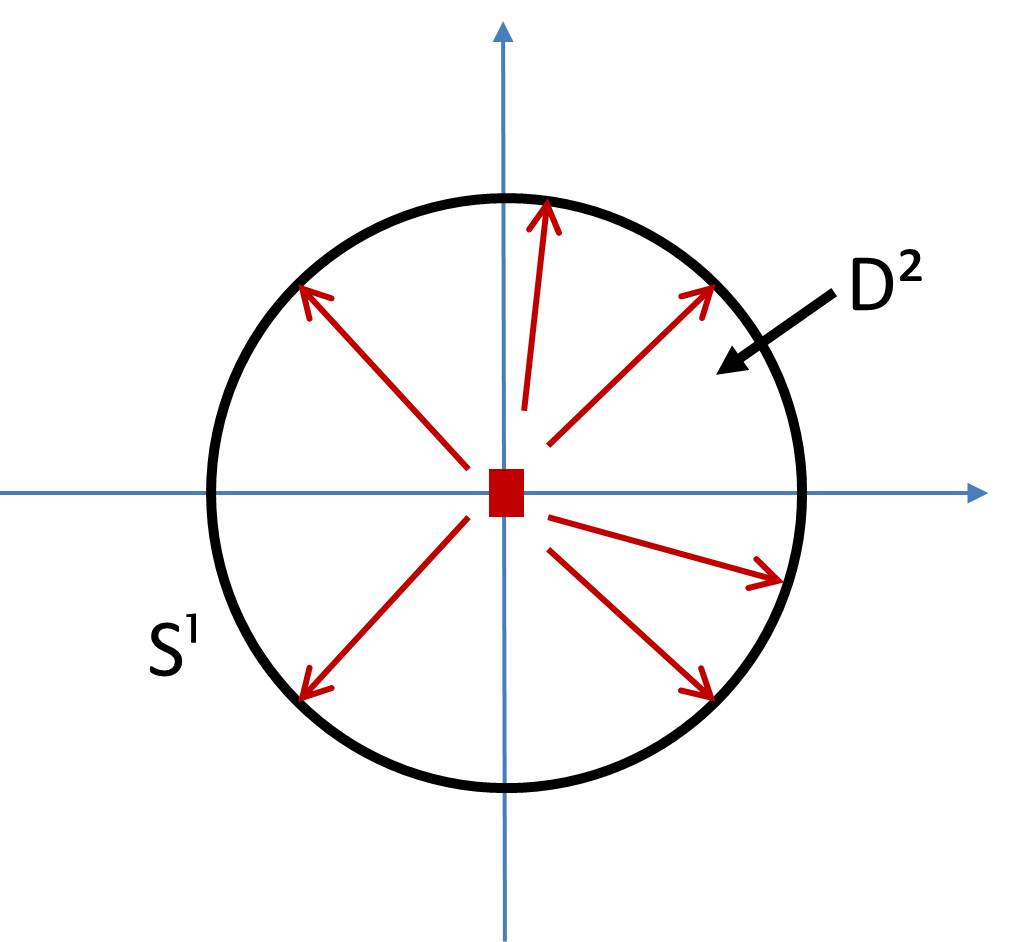
\includegraphics[scale=0.4]{images/Deformationsretrakt_S1_D2.jpg}

\begin{proof}
	Betrachte die Abbildung $$H \colon D^n \backslash \{0\} \times I \rightarrow D^n \backslash \{0\}, (x,t) \mapsto (1-t)x + t \cdot \frac{x}{||x||}$$
	Definiere $r(x)= \frac{x}{||x||}$ für alle $x \in D^n \backslash \{0\}$.
\end{proof}

\chapter{12.12.2011}
\section{Anwendungen zu Sätzen aus der Vorlesung}
\begin{theorem}[Brouwerscher Fixpunktsatz]
	Jede stetige Abbildung $f \colon D^2 \rightarrow D^2$ besitzt einen Fixpunkt, d.h. es ex. $x \in D^2$ mit $f(x)=x$.
\end{theorem}

\paragraph{Fundamentalsatz der Algebra}

\begin{theorem}[Borsuk-Ulam]
	Ist $f \colon S^2 \rightarrow \R^2$ stetig, so existiert ein $x \in S^2$ mit $f(x) = f(-x)$.
\end{theorem}

\begin{corollary}
	Es lässt sich $S^2$ nicht in $\R^2$ einbetten.
\end{corollary}

\begin{corollary}
	Auf der Erde existieren immer zwei verschiedene Punkte mit gleichem Luftdruck und gleicher Temperatur.	
\end{corollary}

\section{Homotopien und Fundamentalgruppe}
\subsection{Der komplex projektive Raum $\C \Prim^n$}
	Der komplex projektive Raum $\C \Prim^n = \{\text{komplexe Geraden durch } 0 \in \C^{n+1}\}$ = $\{\text{1-dim. komplexe lineare Teilräume von } \C^{n+1}\}$ lässt sich auch wie folgt darstellen:
	\newline
	Führt man auf $\C^{n+1} \backslash \{0\}$ durch 
	$$v \sim w :\Leftrightarrow \exists \lambda \in \C \backslash \{0\} \colon \lambda v = w$$
	eine Äquivalenzrelation ein, so kann man $\C \Prim^n$ mit $(\C^{n+1} \backslash \{0\})/_\sim$ identifizieren.
	\newline
	Betrachte $S^{2n+1} = \{v \in \C^{n+1} \mid || v || = 1\}$ als Teilraum von $\C^{n+1}$. Dann induziert die Inklusion $S^{2n+1} \hookrightarrow \C^{n+1} \backslash \{0\}$ einen Homöomorphismus $S^{2n+1} /_\sim \cong (\C^{n+1} \backslash \{0\}) /_\sim$.
	\newline
	Seine Inverse ist die von der radialen Projektion $$\C^{n+1} \backslash \{0\} \rightarrow S^{2n+1}, v \mapsto \frac{1}{||v||} v,$$ induzierte stetige Abbildung $(\C^{n+1} \backslash \{0\})/_\sim \cong S^{2n+1} /_\sim$. 
	\newline
	Da $S^{n+1}$ kompakt ist und die Äquivalenzklassen in $S^{2n+1}$ abgeschlossen sind, ist $\C \Prim^n \cong S^{2n+1} /_\sim$ kompakter Hausdorffraum.  
	\begin{itemize}
		\item \underline{$n = 0$}: $\C \Prim^0 = \{\text{komplexe Geraden durch } 0 \in \C\}$ ist ein einpunktiger Raum.
		\item \underline{$n=1$}: $\C \Prim^1$ ist homöomorph zu $S^3 /_\sim \cong S^2$, und damit gilt: \newline $\pi_1(\C \Prim^1) = \{0\}$, denn nach Vorlesung gilt $\pi_1(S^n) = \{0\}$ für alle $n \geq 2$ und homöomorphe Räume haben isomorphe Fundamentalgruppen.
		\newline
		Der Homöomorphismus ist gegeben durch die folgende Abbildung
		$$\varphi \colon \underbrace{S^3}_{\subseteq \C^2} \rightarrow S^2, \quad (z,w) \mapsto (2 \bar{z} w, |w|^2 - |z|^2),$$
		welche einen Homöomorphismus $S^3 /_\sim \cong S^2$ induziert.
	\end{itemize}

Allgemein gilt: Für alle $n \in \N_0$ ist $\C \Prim^n$ einfach zusammenhängend (da wegzusammenhängend: $\pi_1(\C \Prim^n) = \{0\}$).

\begin{remark}
	Der reell projektive Raum $\R \Prim^n$ ist für \underline{kein} $n \in \N$ einfach zusammenhängend, seine Fundamentalgruppe ist \underline{nicht} trivial.
\end{remark}

\subsection{Die spezielle unitäre Gruppe $SU(n)$}
Für $n \in \N$ betrachte die spezielle unitäre Gruppe $$SU(n) = \{ A \in \C^{n \times n} \mid A^* A = I_n, \det(A) = 1\}$$
($A^*$ bezeichnet die "Adjungierte":  $A^* = \bar{A}^T$) \newline
Es ist $SU(n)$ als Urbild abgeschlossener Mengen unter stetigen Abbildungen abgeschlossen in $\C^{n^2}$. Da die Spalten einer unitären Matrix orthonormal zueinander sind und somit Einheitsvektoren bilden, ist $SU(n)$ beschränkt. Nach dem Satz von Heine-Borel (welcher anwendbar ist, da $\C^{n^2} \cong \R^{2n^2}$) ist $SU(n)$ damit kompakt.
\begin{itemize}
	\item \underline{$n=1$}: $SU(1) = \{ z \in \C, \bar{z}z = 1, \det(z) = 1\} = \{1\}$ ist ein einpunktiger Raum.
	\item \underline{$n=2$}: $SU(2)$ ist homöomorph zu $S^3$ und damit einfach zusammenhängend (mit gleicher Begründung wie für $\C \Prim ^1$). \newline
	Zum Homöomorphismus:
	\newline
	Betrachte $S^3 = \{(z,w) \in \C^2 \mid |z|^2 + |w|^2 = 1 \}$ als Teilraum von $\C^2$.
	Dann ist
		$$\varphi \colon S^3 \rightarrow SU(2), \quad (z,w) \mapsto \begin{pmatrix}
		z & -\bar{w} \\ w & \bar{z}
		\end{pmatrix} $$
	ein Homöomorphismus $S^3 \cong SU(2)$.
	\item Allgemein gilt: Für jedes $n \in \N$ ist $SU(n)$ einfach zusammenhängend.
\end{itemize}

\subsection{Die Kreislinie $S^1 \subseteq \R^2$}

\begin{beh}
	$S^1$ ist nicht einfach zusammenhängend.
	\begin{figure}[h]
	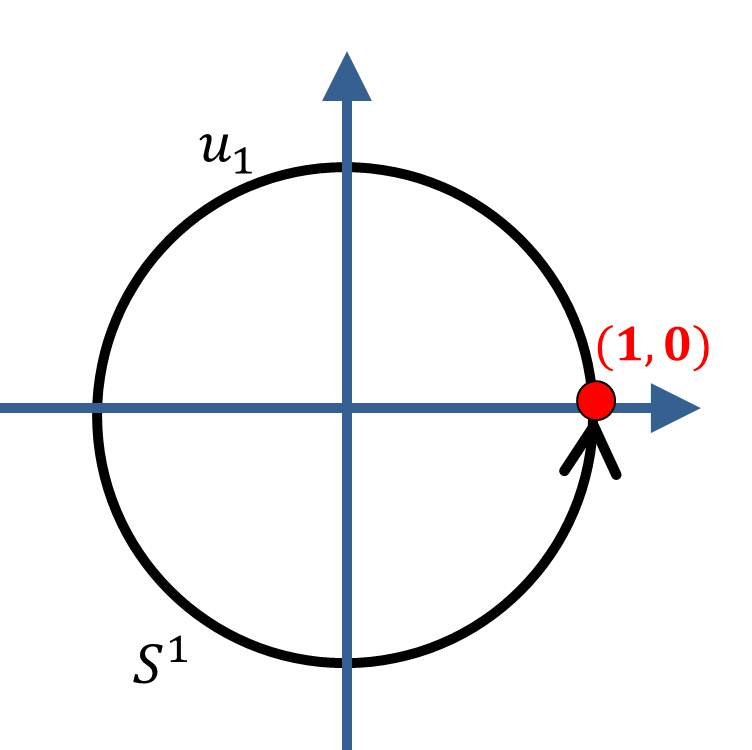
\includegraphics[scale=0.4]{images/S1_nichttrivialer_Weg.jpg}
	\end{figure}
\end{beh}
Was sind geschlossene Wege in $S^1$?
\newline
Für $ k \in \Z$ definiere
$$u_k \colon I \rightarrow S^1, \quad t \mapsto (\cos 2 \pi k t, \sin 2 \pi k t)$$
Solche Schleifen lassen sich für $k \neq 0$ nicht zusammenziehen.

\subsection{Das Möbiusband}
Das Möbiusband $M$ entsteht durch Verklebung zweier gegenüberliegender Seiten im Einheitsquadrat $I^2$ in entgegengesetzter Richtung:
$$M = I^2/_{[(0,t) \sim (1, 1-t)]}$$
	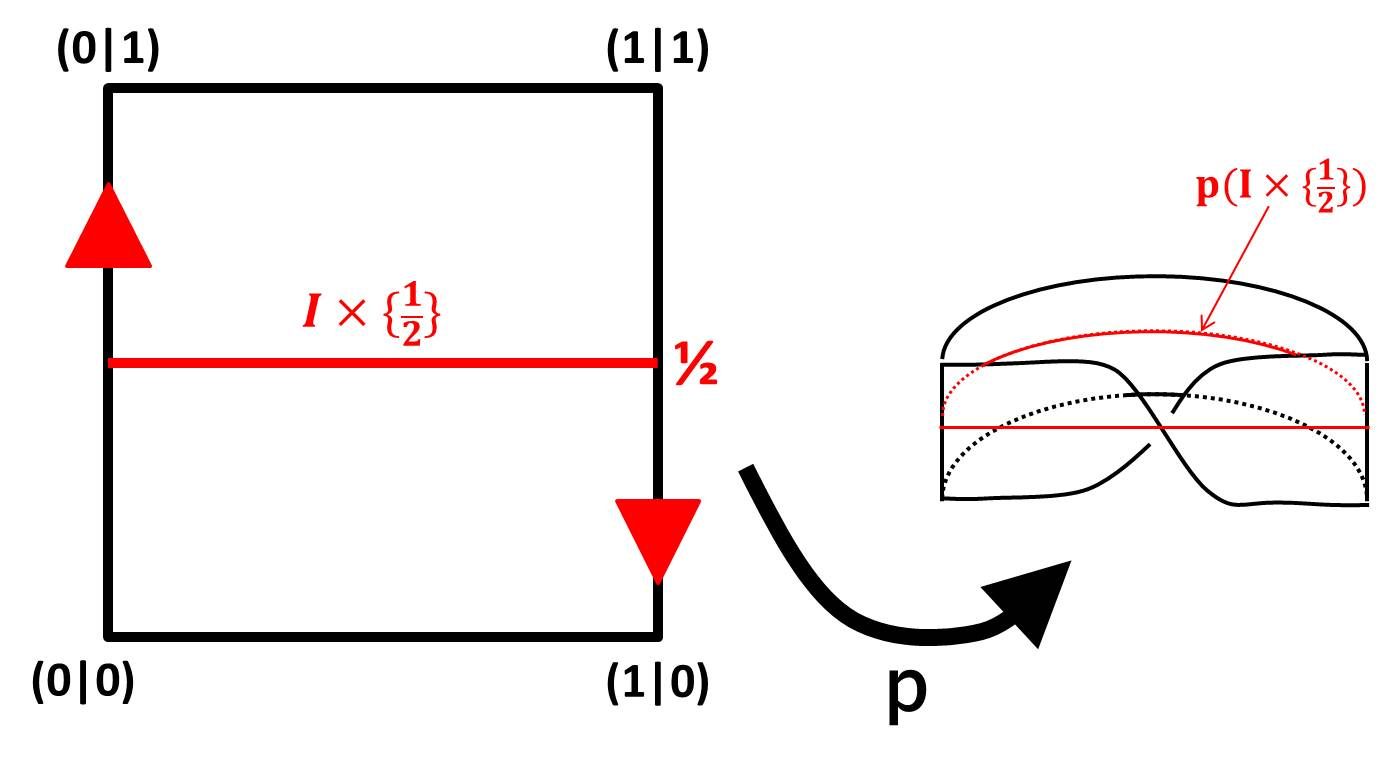
\includegraphics[scale=0.4]{images/Moebiusband.jpg}
\newline
Es bezeichnet $p \colon I^2 \rightarrow M$ die Projektion und $S:= p(I \times \{\frac{1}{2}\})$.

Man kann zeigen, dass $S$ ein Deformationsretrakt von $M$ ist.
\newline
Somit sind $S$ und $M$ vom selben Homotopietyp und damit $$\pi_1(M) \underbrace{\approx}_{\text{isomorph}} \pi_1(S).$$
Andererseits gilt: $S$ ist homöomorph zu $S^1$ und somit: 
$$\pi_1(S^1) \approx \pi_1(S) \approx \pi_1(M).$$

\chapter{19.12.2011}
\section{Überlagerungen und Liftungen}

\begin{definition}
	Eine Überlagerung eines topologischen Raumes $X$ ist ein Raum $\widetilde{X}$ zusammen mit einer surjektiven stetigen Abbildung $\pi \colon \widetilde{X} \rightarrow X$, so dass für alle Punkte $x \in X$ eine Umgebung $U=U(x)$ existiert mit
	\begin{enumerate}
		\item $\pi^{-1}$ ist eine nichtleere Vereinigung paarweise disjunkter offener Mengen $\widetilde{U_j} \subseteq \widetilde{X}, j \in J$,
		\item Für alle $j \in J$ ist $\pi \big |_{\widetilde{U_j}} \colon \widetilde{U_j} \rightarrow U$ ein Homöomorphismus.
	\end{enumerate}
\end{definition}

[$\pi$ \underline{Überlagerungsabbildung}, $|J|$ \underline{Blätterzahl}, $\widetilde{X}$ \underline{Totalraum}, $X$ \underline{Basisraum}, $\pi^{-1}(x)$ \underline{Faser über $x$} (für $x \in X$)]

\begin{center}
	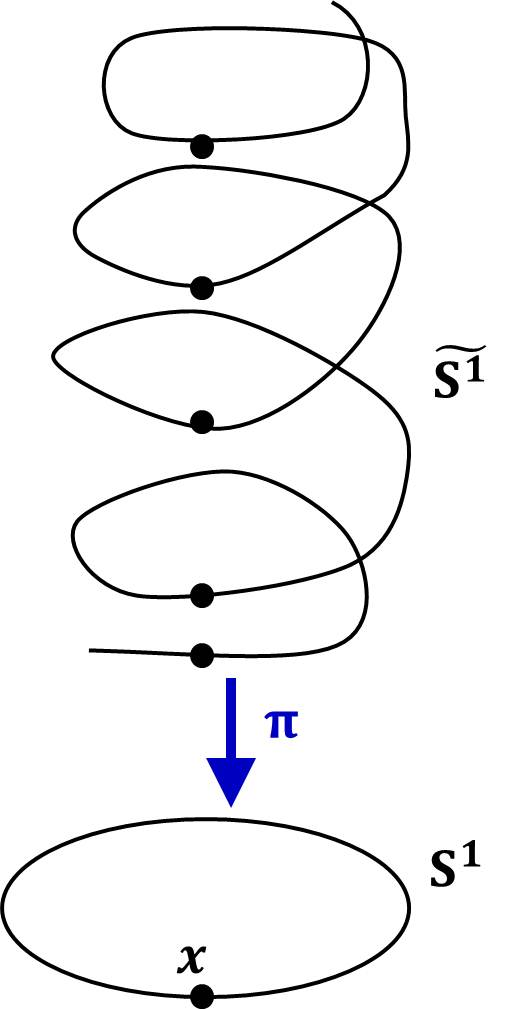
\includegraphics[scale=0.5]{images/2011_12_19_Bild1.jpg}
\end{center}

\begin{definition}[Lift]
	Ist $\pi \colon \widetilde{X} \rightarrow X$ eine Überlagerung, $f \colon [0,1] \rightarrow X$ ein Weg, so heißt $\widetilde{f} \colon [0,1] \rightarrow \widetilde{X}$ \underline{Lift} von $f$, falls $\pi \circ \widetilde{f} = f$ gilt.
\end{definition}

\begin{center}
	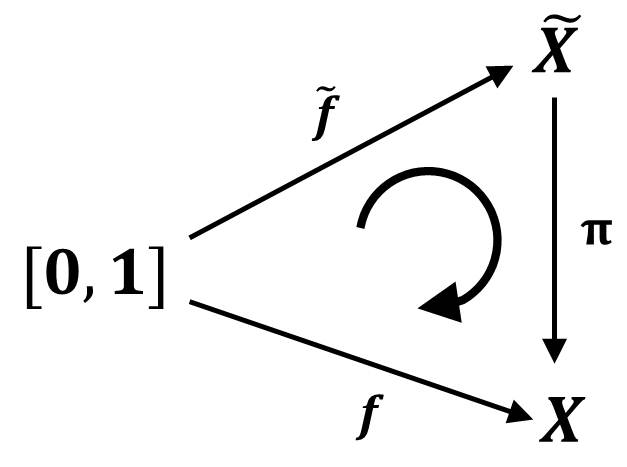
\includegraphics[scale=0.5]{images/2011_12_19_Bild2.jpg}
\end{center}

\section{Folgerungen aus dem Satz über das Hochheben von Homotopien}
\begin{corollary}
	Es sei $X$ ein topologischer Raum, $\pi \colon \widetilde{X} \rightarrow X$ eine Überlagerung, $x_0 \in X, \widetilde{x_0} \in \pi^{-1}(x_0)$. Weiter sei $f \colon S^1 \rightarrow X$ eine Schleife in $x_0$ und $\widetilde{f}$ der Lift von $f$ mit Anfangspunkt $\widetilde{x_0}$. Dann gilt:
	$$\widetilde{f} \text{ ist Schleife } \Leftrightarrow [f] \in \pi_*(\pi_1(\widetilde{X}, \widetilde{x_0})),$$
	wobei $\pi_* \colon \pi_1(\widetilde{X}, \widetilde{x_0}) \rightarrow \pi_1(X,x_0)$ die induzierte Abbildung bezeichne.
\end{corollary}

\begin{proof}
	\underline{$"\Rightarrow"$:} Es sei $\widetilde{f}$ eine Schleife (d.h. ein \underline{geschlossener} Weg). Dann ist $[\widetilde{f}] \in \pi_1(\widetilde{X}, \widetilde{x_0})$ und somit:
	$$[f] = [\pi \circ \widetilde{f}] = \pi_*([\widetilde{f}]) \in \pi_*(\pi_1(\widetilde{X}, \widetilde{x_0})).$$
	\underline{$"\Leftarrow"$:} Es sei $[f] \in \pi_*(\pi_1(\widetilde{X}, \widetilde{x_0}))$.
	\newline
	Es sei $\widetilde{g}$ eine Schleife in $\widetilde{x_0}$ mit
	$$[f] = \pi_*([\widetilde{g}]) = [\pi \circ \widetilde{g}].$$
	Dann sind $f$ und $\pi \circ \widetilde{g}$ homotop vermöge einer Homotopie $H \colon f \simeq \pi \circ \widetilde{g}$. Es sei $H$ der Lift von $H$ mit $\widetilde{H_0} = \widetilde{f}$, $\widetilde{H_1} = \widetilde{g}$.
	\newline
	Nach dem Monodromie-Lemma haben alle Wege $\widetilde{H_t}$ den gleichen Endpunkt. Damit folgt:
	$$\widetilde{f}(0) = \widetilde{x_0} = \widetilde{g}(1) = \widetilde{H_1}(1) \overset{\text{Monodromie-Lemma}}{=} \widetilde{H_0}(1) = \widetilde{f}(1).$$
	Also ist $\widetilde{f}$ eine Schleife (in $\widetilde{x_0}$).
\end{proof}

\begin{corollary}
	Es sei $X$ ein wegzusammenhängender topologischer Raum, der eine wegzusammenhängende nichttriviale Überlagerung $\pi \colon \widetilde{X} \rightarrow X$ besitze (d.h. $\pi$ ist mindestens zweiblättrig). Ist $x_0 \in X$, so gilt:
	$$\pi_1(X,x_0) \neq \{1\}.$$
\end{corollary}

\begin{proof}
	Sei $x_0 \in X$. Es seien $\widetilde{x_1}, \widetilde{x_2} \in \pi^{-1}(x_0)$ mit $\widetilde{x_1} \neq \widetilde{x_2}$. Ferner sei
	$$\gamma \colon [0,1] \rightarrow \widetilde{X}$$ ein Weg von $\widetilde{x_1}$ zu $\widetilde{x_2}$.
	
\begin{center}
	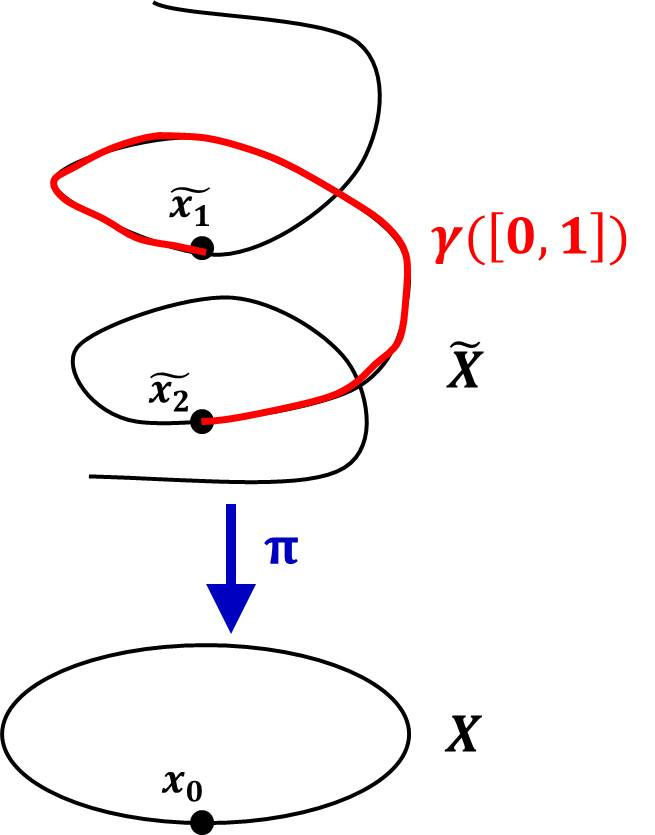
\includegraphics[scale=0.5]{images/2011_12_19_Bild3.jpg}
\end{center}
	Dann ist $\pi \circ \gamma$ ein geschlossener weg in $X$, der sich \underline{nicht} in einen geschlossenen Weg liften lässt. es gilt also: $\pi \circ \gamma \in \pi_1(X,x_0)$. Nach obigem Korollar gilt aber: Der Lift von $\pi \circ \gamma$ ist nicht im Bild von $\pi_*(\pi_1(\widetilde{X}, \widetilde{x_0}))$. Somit gibt es ein Element in $\pi_1(X,x_0)$, welches nicht im Bild der induzierten Abbildung 
	$$\pi_* \colon \pi_1(\widetilde{X}, \underbrace{\widetilde{x_0}}_{\in \pi^{-1}(x_0)}) \rightarrow \pi_1(X,x_0)$$ liegt.
	\newline
	Da $\pi_*$ ein Gruppenhomomorphismus ist, gilt sicher: $1 \in \pi_*(\pi_1(\widetilde{X},\widetilde{x_0}))$.
	\newline
	Also folgt: $\pi_1(X,x_0) \neq \{1\}$.
\end{proof}

\begin{example}
	Die kanonische Projektion $S^2 \rightarrow S^2/_{[x \sim (-x)]} = \R \Prim^2$ ist eine zweiblättrige Überlagerung. 
\begin{center}
	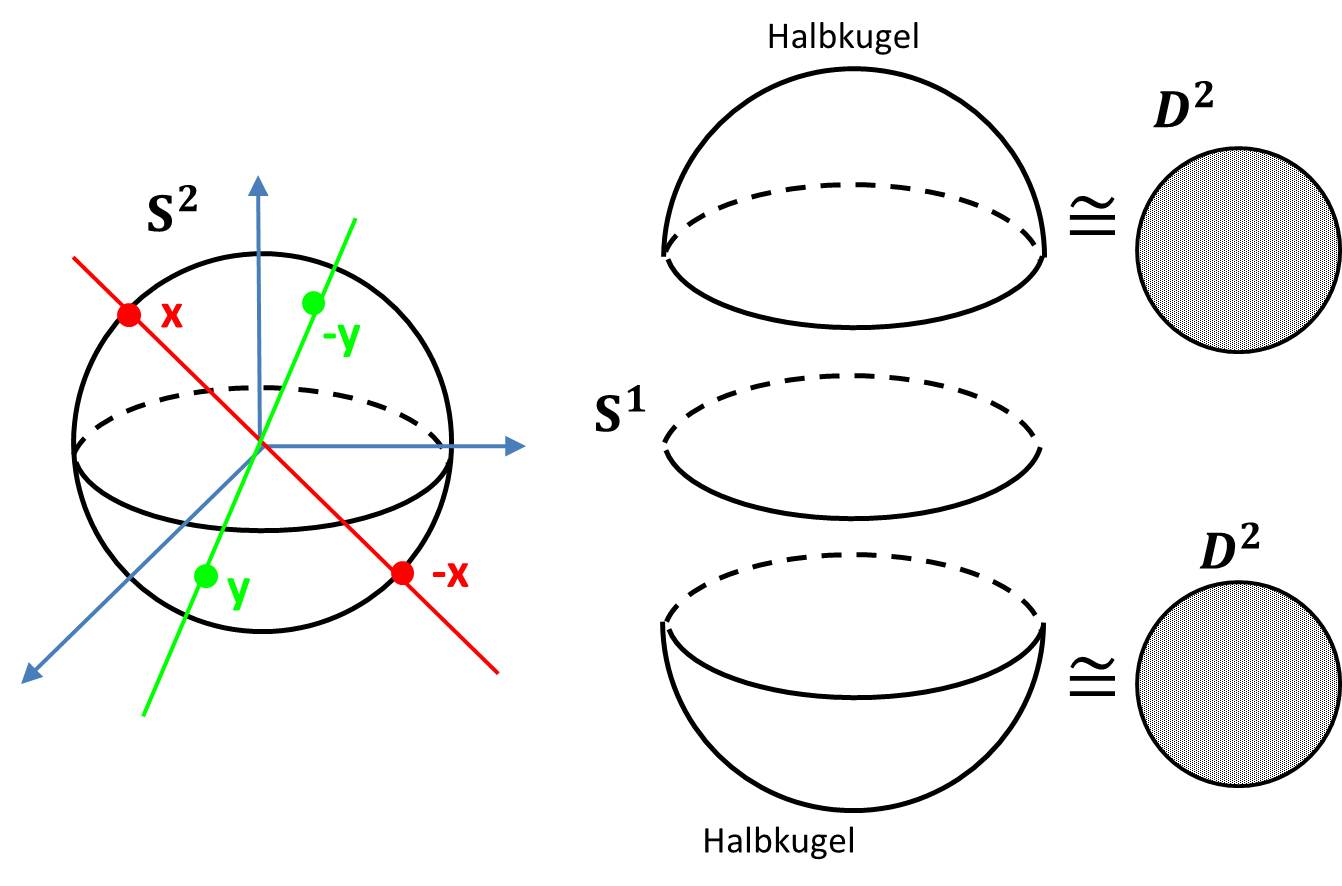
\includegraphics[scale=0.5]{images/2011_12_19_Bild4.jpg}
\end{center}
	Es sind sowohl $S^2$ als auch $\R \Prim^2$ wegzusammenhängend. Dann folgt mit dem Korollar: 
	$$\pi_1(\R \Prim^2) \neq \{1\} \text{ (zu jedem beliebigen Basispunkt)}.$$
	Nach Vorlesung ist $S^2$ einfach zusammenhängend (d.h. wegzusamenhängend und mit trivialer Fundamentalgruppe). Da homöomorphe Räume isomorphe Fundamentalgruppen haben, können also $S^2$ und $\R \Prim^2$ nicht homöomorph sein.
\end{example}

\begin{example}
	Der Torus ist eine zweiblättrige Überlagerung der Kleinschen Flasche.
	
\begin{center}
	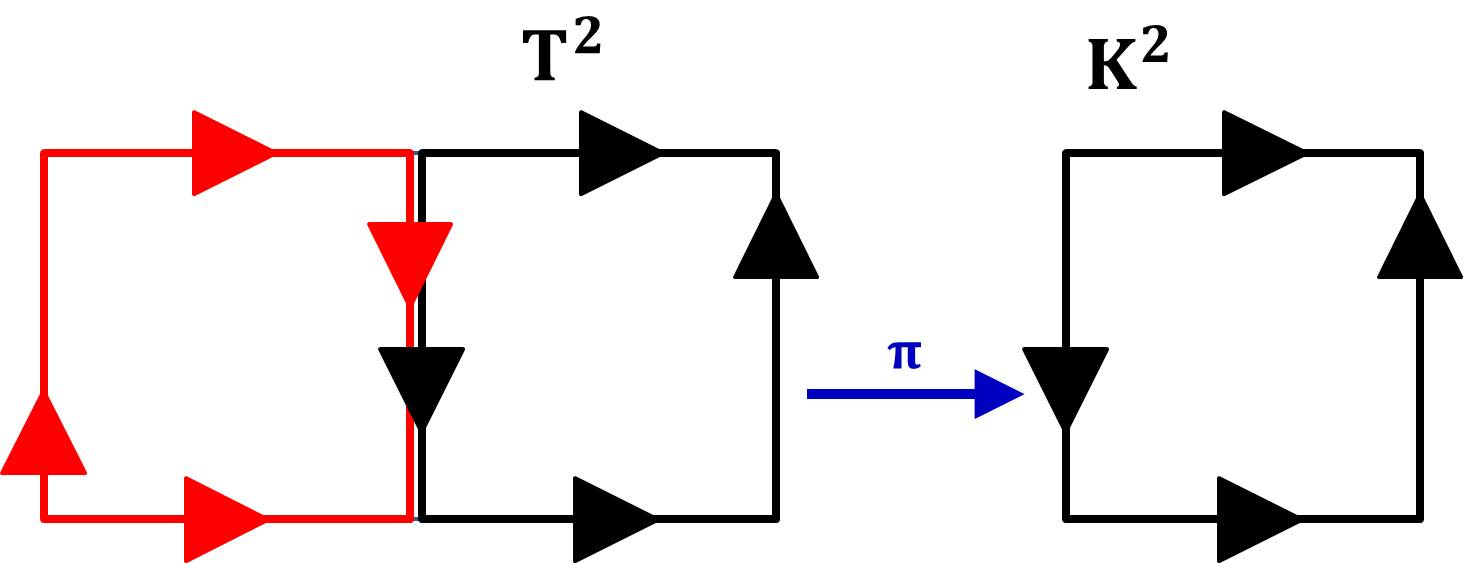
\includegraphics[scale=0.5]{images/2011_12_19_Bild5.jpg}
\end{center}
\end{example}

\chapter{09.01.2012}

\section{Überlagerungen und Decktransformationen}

\begin{definition}[lokal wegzusammenhängend]
	Ein topologischer Raum $X$ heißt \underline{lokal wegzusammenhängend}, falls jede offene Umgebung $U$ eines Punktes $x \in X$ eine wegzusammenhängende Umgebung enthält, d.h. $\forall x \in X \quad \forall U = U(x) \quad \exists V \subseteq U \colon x \in V \text{ und } V \text{ wegzusammenhängend}.$
\end{definition}

\begin{remark}
	Ein lokal wegzusammenhängender Raum ist genau dann wegzusammenhängend, wenn er zusammenhängend ist.
\end{remark}

\begin{example}
	
\begin{center}
	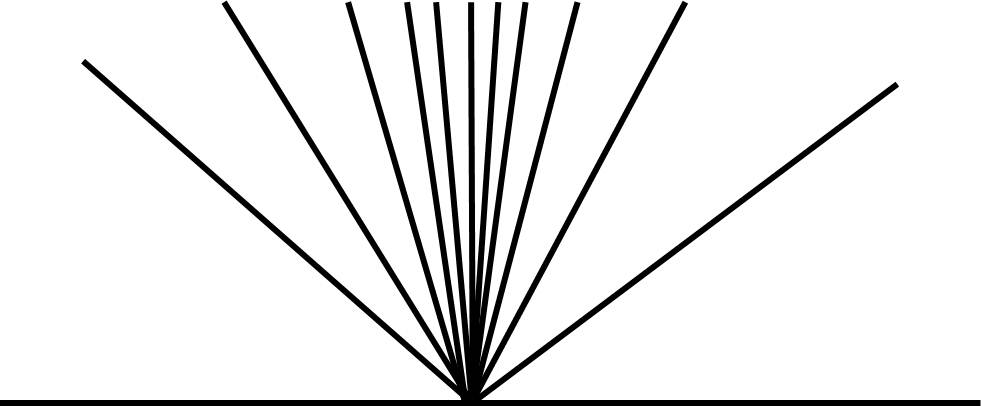
\includegraphics[scale=0.5]{images/2012_01_09_Bild1.jpg}
\end{center} Wegzusammenhängend, aber nicht lokal wegzusammenhängend.
\end{example}

\begin{definition}[Decktransformation]
	Sei $X$ ein topologischer Raum. Eine \underline{Decktransformation} (oder \underline{-bewegung}) einer Überlagerung $\pi \colon \widetilde{X} \rightarrow X$ ist ein Homöomorphismus $d \colon \widetilde{X} \rightarrow \widetilde{X}$ mit $\pi = \pi \circ d$. \begin{center}
	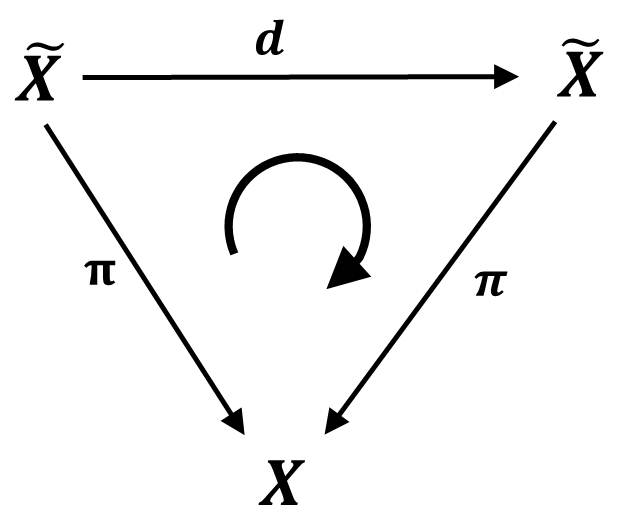
\includegraphics[scale=0.5]{images/2012_01_09_Bild2.jpg}
\end{center}
	(Alternativ: Decktransformationen überlagern die Identität $X \rightarrow X$. \begin{center}
	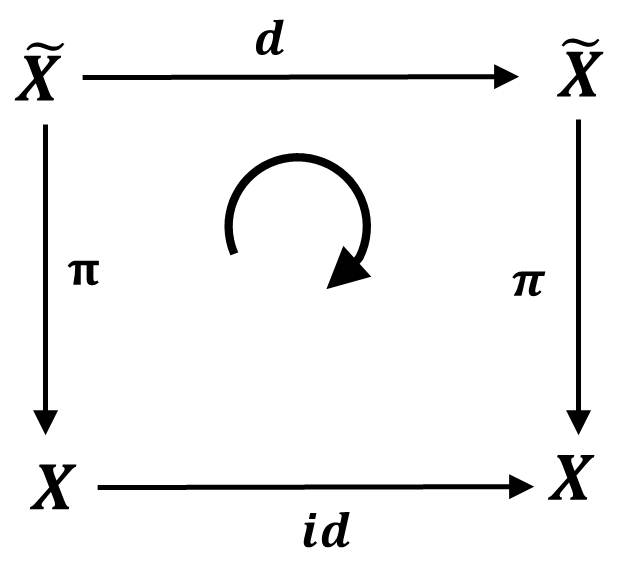
\includegraphics[scale=0.5]{images/2012_01_09_Bild3.jpg}
\end{center})
\end{definition}

\begin{example}
	\begin{itemize}
		\item Für $\pi \colon \R \rightarrow S^1, t \mapsto e^{2 \pi i t}$, sind die Deckbewegungen die ganzzahligen Translationen $\R \rightarrow \R, x \mapsto x + z$ mit $z \in \Z$; und für die Deckbewegungsgruppe erhält man $D \cong \Z$.
		\item Für $\pi \colon \R^2 \rightarrow S^1 \times S^1 \cong T^2$ sind die Deckbewegungen die Translationen $\R^2 \rightarrow \R^2, (x,y) \mapsto (x+m, y+n)$ für $m,n \in \Z$; und es gilt: $D \cong \Z \times \Z$.
		\item Für $\pi \colon S^1 \rightarrow S^1, z \mapsto z^n$ für $n \in \N$ sind die Deckbewegungen Drehungen um ein Vielfaches des Winkels $\frac{2 \pi}{n}$; und es gilt: $D \cong \Z /_{n \Z}$.
	\end{itemize}
\end{example}

\section{Einschub Gruppenoperationen}
\paragraph{Erinnerung}
Eine \underline{topologische Gruppe} ist eine Gruppe $G$, die zugleich ein topologischer Raum ist, so dass
$$G \times G \rightarrow G, (g,h) \mapsto gh,$$
$$G \rightarrow G, g \mapsto g^{-1}$$
stetig sind.

Es seien $G$ eine topologische Gruppe, $X$ ein topologischer Raum.
\begin{definition}
	\begin{itemize}
		\item Eine \underline{Operation} oder \underline{Wirkung} von $G$ auf $X$ ist eine stetige Abbildung 
		$$G \times X \rightarrow X, (g,x) \mapsto g. x$$
		mit folgenden Eigenschaften:
		\begin{enumerate}
			\item $\forall x \in X \colon e. x = x$ für das neutrale Element $e \in G$;
			\item $\forall x \in X \quad \forall g_1, g_2 \in G \colon g_1.(g_2.x) = (g_1g_2).x$
		\end{enumerate}
		
		\item Die Menge $G.x = \{ g.x \mid g \in G\}$ heißt \underline{Orbit} oder \underline{Bahn} von $x$ unter $G$.
		
		\item $G$ operiert \underline{transitiv} auf $X$, falls für alle $x,y \in X$ ein $g \in G$ existiert mit $g.x = y$.
		
		\item $G$ operiert \underline{eigentlich diskontinuierlich} auf $X$, falls zu jedem $x \in X$ eine Umgebung $U(x) = U$ existiert mit $g.U \cap U = \emptyset$ für alle $g \in G \backslash \{e\}$.
		\newline
		(Dann ist auch $g.U \cap g^\prime.U = \emptyset$ für alle $g, g^\prime \in G$ mit $g \neq g^\prime$.)
	\end{itemize}
\end{definition}

\begin{theorem}
	Es sei $X$ ein topologischer Raum, auf dem eine topologische Gruppe $G$ eigentlich diskontinuierlich wirkt. Dann ist $\pi \colon X \rightarrow X/_G$ auf den sogenannten \underline{Orbit-} oder \underline{Bahnenraum} $X/_G$ eine Überlagerung, deren Blätterzahl der Mächtigkeit von $G$ entspricht.
\end{theorem}

\begin{proof}
	Für $x \in X$ sei $U$ eine Umgebung von $x$ mit $g.U \cap g^\prime.U = \emptyset$ für alle $g,g^\prime \in G$ mit $g \neq g^\prime$.
	\newline
	Dann ist $V = \pi(U) \subseteq X/_G$ eine \begin{center}
	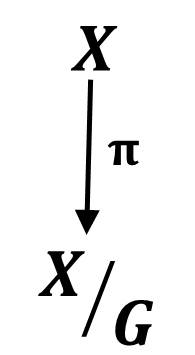
\includegraphics[scale=0.5]{images/2012_01_09_Bild4.jpg}
\end{center} überlagerte Umgebung von $\pi(x)$ in $X/_G$ (da $\pi^{-1}(V) = \bigcup\limits_{g \in G}^\cdot {g.U} \text{ (disjunkte Vereinigung)}$.)
	\newline
	Die Blätter über $V$ sind die offenen Mengen $g.U$ für $g \in G$.
\end{proof}

\begin{example}
	Die Gruppe $\Z^n$ operiert auf $\R^n$ durch $(a,x) \mapsto a+x$ eigentlich diskontinuierlich.
	\newline
	Daher ist $\pi \colon \R^n \rightarrow \R^n /_{\Z^n} \cong T^n$ eine unendlich-blättrige Überlagerung.
	\newline
	Es sei $f \colon \R^n/_{\Z^n} \rightarrow \underbrace{S^1 \times \ldots \times S^1}_{n \text{ Faktoren}}$ der Homöomorphismus $$\pi(x_1, \ldots, x_n) \mapsto (e^{2 \pi i x_1}, \ldots, e^{2 \pi i x_n})$$
	Dann ist $f \circ \pi \colon \R^n \rightarrow S^1 \times \ldots \times S^1$ ebenfalls eine Überlagerung.
\end{example}
Verschärfung des Satzes:

\begin{theorem}
	Wirkt eine topologische Gruppe $G$ eigentlich diskontinuierlich auf einen wegzusammenhängenden und lokal wegzusammenhängenden topologischen Raum $X$, so ist die Projektion $\pi \colon X \rightarrow X/_G$ eine \underline{reguläre} Überlagerung mit Deckbewegungsgruppe $D=G$.
\end{theorem}

\begin{definition}[reguläre/normale Überlagerung]
	Eine Überlagerung $\pi \colon \widetilde{X} \rightarrow X$ heißt \underline{regulär} (oder \underline{normal}), falls die Deckbewegungsgruppe transitiv auf $\pi^{-1}(x)$ für $x \in X$ operiert.
\end{definition}

\begin{definition}[semilokal einfach zusammenhängend]
	Ein topologischer Raum heißt \underline{semilokal einfach zusammenhängend}, falls für jeden Punkt $x \in X$ eine Umgebung $U=U(x)$ existiert, so dass jeder in $U$ liegende geschlossene Weg \underline{in $X$} nullhomotop ist.
\end{definition}

\begin{theorem}[Klassifikationssatz für Überlagerungen]
	Es sei $X$ ein wegzusammenhängender, lokal wegzusammenhängender und semilokal einfach zusammenhängender topologischer Raum, der eine einfach zusammenhängende (d.h. eine sogenannte \underline{universelle}) Überlagerung besitze.
	\newline
	Die Äquivalenzklassen der Überlagerungen mit Basispunkten, die auf $x_0 \in X$ abgebildet werden, entsprechen bijektiv den Untergruppen von $\pi_1(X,x)$.
\end{theorem}

(Die Bijektion ist gegeben durch $\widetilde{X} \leftrightarrow \pi_*(\pi_1(\widetilde{X}))$ für eine Überlagerung $\pi \colon \widetilde{X} \rightarrow X$.)

\begin{example}
	Die Untergruppen von $\pi_1(S^2) \cong \Z$ sind $n \Z$ für $n \in \N \cup \{0\}$.
	\newline
	Die zugehörigen Überlagerungen sind 
	$$\pi \colon \R \rightarrow S^1, t \mapsto e^{2 \pi i t} \text{ für } n = 0,$$
	$$\pi_n \colon S^1 \rightarrow S^1, z \mapsto z^n \text{ für } n \geq 1.$$
\end{example}

\begin{definition}[universelle Überlagerung]
	Für einen wegzusammenhängenden Raum $X$ heißt eine Überlagerung $\pi \colon \widetilde{X} \rightarrow X$ \underline{universell}, falls $\widetilde{X}$ einfach zusammenhängend ist.
\end{definition}

\paragraph{Warum "universell"?}
Eine einfach zusammenhängende Überlagerung überlagert selbst wieder jede andere Überlagerung und alle einfach zusammenhängenden Überlagerungen sind äquivalent.

\paragraph{Hauptresultat}
Jeder wegzusammenhängende, lokal wegzusammenhängende und semilokal einfach zusammenhängende topologische Raum besitzt eine universelle Überlagerung!

\chapter{23.01.2012}
\section{Geometrie von Flächen}

\begin{definition}[Fläche in $\R^3$]
	Eine \underline{Fläche in $\R^3$} ist eine glatte, 2-dimensionale Untermannigfaltigkeit von $\R^3$.
\end{definition}

\begin{remark}{}
	$F \subset \R^3$ ist Fläche im $\R^3$ genau dann, wenn für jeden Punkt $x \in F$ eine Umgebung $U=U(x) \subseteq F$ existiert und $r \colon V \rightarrow \R^3$ für eine Umgebung $V \subset \R^2$, so dass gilt:
	\begin{enumerate}
		\item $r \colon V \rightarrow U$ ist Homöomorphismus,
		\item $r(u,v) = (x(u,v), y(u,v), z(u,v))$ ist glatt,
		\item $r_u := \frac{\partial r}{\partial u} = \left ( \frac{\partial x}{\partial u}, \frac{\partial y}{\partial u}, \frac{\partial z}{\partial u} \right )$ und $r_v := \frac{\partial r}{\partial v} = \left ( \frac{\partial x}{\partial v}, \frac{\partial y}{\partial v}, \frac{\partial z}{\partial v} \right )$ sind in jedem Punkt \footnote{von $V$} linear unabhängig.
	\end{enumerate}
\end{remark}

\begin{example}{}
\begin{itemize}
	\item Torus:
	\newline
	Eine Parameterdarstellung des Torus ist für $a,b > 0$ gegeben durch
	$$r(u,v) = (a + b \cdot \cos u) (\cos v \cdot e_1 + \sin v \cdot e_2) + b \cdot \sin u \cdot e_3$$
	\item Allgem. Rotationsfläche: \newline
	$$r(u,v) = f(u) (\cos v \cdot e_1 + \sin v \cdot e_2) + u \cdot e_3$$
	$\Rightarrow$ Spezialfall: Zylinder
	$$r(u,v) = a (\cos v \cdot e_1 + \sin v \cdot e_2) + u \cdot e_3$$
	$$= (a \cdot \cos v, a \cdot \sin v, u)$$
\end{itemize}
\end{example}

\begin{definition}[Bogenlänge einer glatten Kurve]
	Die \underline{Bogenlänge} einer glatten Kurve $\gamma \colon [a,b] \rightarrow F$ in $F$ ist gegeben durch
	$$L(\gamma) = \int\limits_a^b{|\gamma^\prime(t)|} dt = \int\limits_a^b{\sqrt{\gamma^\prime \cdot \gamma^\prime} dt} = \int\limits_a^b{\sqrt{(r_u u^\prime + r_v v^\prime) \cdot (r_u u^\prime + r_v v^\prime)} dt}$$
	$$= \int\limits_a^b{\sqrt{E \cdot (u^\prime)^2 + 2 F \cdot u^\prime v^\prime + G \cdot (v^\prime)^2} dt}$$ mit $E:= r_u \cdot r_u, F:= r_u \cdot r_v, G := r_v \cdot r_v$.
\end{definition}

\begin{definition}[erste Fundamentalform]
	Die \underline{erste Fundamentalform} einer Fläche im $\R^3$ ist gegeben durch
	$$\RM{1} := E \cdot d u^2 + 2 F \cdot du \cdot dv + G \cdot dv^2$$ mit $E,F,G$ wie oben.
\end{definition}

\begin{example}[Erste Fundamentalform des Zylinders]
	Parametrisierung des Zylinders ist gegeben durch
	$$r(u,v) = (a \cdot \cos v, a \cdot \sin v, u).$$
\end{example}
\footnote{Hinweis: Fundamentalform ausrechnen lassen könnte in der Klausur drankommen.}
Es gilt:
$$r_u = \frac{\partial r}{\delta u} = (0,0,1),$$
$$r_v = \frac{\partial r}{\partial u} = (-a \cdot \sin v, a \cdot \cos v, 0).$$
Damit folgt:
$$E = r_u \cdot r_u = 1,$$
$$F = r_u \cdot r_v = 0,$$ \footnote{Hier überall Skalarprodukt!}
$$G = r_v \cdot r_v = a^2.$$
Also gilt für die erste Fundamentalform:
$$\RM{1}_\text{Zylinder} = E du^2 + 2 F dudv + G dv^2$$
$$= du^2 + a^2 dv^2$$

\paragraph{Die Sphäre $S^2 \subseteq \R^3$}
Eine Parameterdarstellung der Sphäre $S^2$ ist gegeben durch
$$r(u,v) = (a \cdot \cos u \cos v, a \cdot \sin u \cos v, a \cdot \sin v)$$
(für $a>0, u \in [0,2 \pi], v \in \left[ - \frac{\pi}{2}, \frac{\pi}{2} \right]$).

Für die Tangentialvektoren $r_u$ und $r_v$ gilt:
$$r_u = \frac{\partial r}{\partial u} = (- a \cdot \sin u \cos v, a \cdot \cos u \cos v, 0)$$
$$r_v = \frac{\partial r}{\partial v} = (- a \cdot \cos u \sin v, -a \cdot \sin u \sin v, a \cdot \cos v)$$

Der Tangentialraum $T_x S^2$ im Punkte $x \in S^2$ ist der Aufspann von $(r_u\circ r^{-1})(x)$ und $(r_v\circ r^{-1})(x)$.

\paragraph{(Einheits-) \underline{Normalenvektoren}}
Es gilt:
$$r_u \times r_v = \begin{pmatrix}
- a \cdot \sin u \cos v \\ a \cdot \cos u \cos v \\ 0
\end{pmatrix} \times \begin{pmatrix}
- a \cdot \cos v \sin v \\ -a \cdot \sin u \sin v \\ a \cdot \cos v
\end{pmatrix} = a^2 \begin{pmatrix}
\cos u \cos^2 v \\ \sin u \cos^2 v \\ \sin v \cos v
\end{pmatrix}.$$ \footnote{Muss (für Einheitsnormalenvektoren) noch durch die Norm geteilt werden}
\newline
\hrulefill
\newline \paragraph{Wiederholung Kreuzprodukt}
für $a,b \in \R^3$ gilt:
$$\begin{pmatrix}
a_1 \\ a_2 \\ a_3
\end{pmatrix} \times \begin{pmatrix}
b_1 \\ b_2 \\ b_3
\end{pmatrix} = \begin{pmatrix}
a_2b_3 - a_3b_2 \\ a_3b_1 - a_1 b_3 \\ a_1 b_2 - a_2 b_1
\end{pmatrix}$$

\paragraph{Erste Fundamentalform}
Es gilt:
$$E = r_u \cdot r_u = a^2 \cdot \cos^2 v,$$
$$F = r_u \cdot r_v = 0,$$
$$G = r_v \cdot r_v = a^2.$$

Damit folgt für die erste Fundamentalform:
$$\RM{1}_\text{Sphäre} = E du^2 + 2 F du dv + G dv^2 = a^2 \cdot \cos^2 v du^2 + a^2 dv^2$$


\end{document}
